\documentclass[10pt]{article}

% ── Packages ─────────────────────────────────────────────────────────────────
\usepackage[margin=1.2in,top=1in,bottom=1.1in]{geometry}
\usepackage{amsmath,amssymb,amsthm}
\theoremstyle{plain}
\newtheorem{theorem}{Theorem}[section]
\newtheorem{proposition}[theorem]{Proposition}
\newtheorem{corollary}[theorem]{Corollary}
\newtheorem{lemma}[theorem]{Lemma}
\theoremstyle{definition}
\newtheorem{definition}[theorem]{Definition}
\newtheorem{remark}[theorem]{Remark}
\usepackage{graphicx}
\usepackage{booktabs}
\usepackage{colortbl,xcolor}
\usepackage[hidelinks]{hyperref}
\usepackage{subcaption}
\usepackage{placeins}
\usepackage{tikz}
\usetikzlibrary{arrows.meta,shapes.geometric,positioning,fit,
                calc,decorations.pathreplacing,patterns,backgrounds}
\usepackage{algorithm}
\usepackage{algpseudocode}

\usepackage{cite}
\usepackage{enumitem}
\setlist{noitemsep,topsep=2pt}

\definecolor{ours}{RGB}{220,235,255}

%── DeepMind palette (Figure 2) ──────────────────────────────────────────────
\definecolor{dmBlue}{HTML}{1A73E8}
\definecolor{dmBlueL}{HTML}{E8F0FE}
\definecolor{dmTeal}{HTML}{00897B}
\definecolor{dmTealL}{HTML}{E0F2F1}
\definecolor{dmGreen}{HTML}{34A853}
\definecolor{dmGreenL}{HTML}{E6F4EA}
\definecolor{dmAmber}{HTML}{E37400}
\definecolor{dmAmberL}{HTML}{FEF3CD}
\definecolor{dmGray}{HTML}{5F6368}
\definecolor{dmGrayL}{HTML}{F1F3F4}
\definecolor{dmGrayM}{HTML}{DADCE0}
\definecolor{dmText}{HTML}{202124}
% ── Title ─────────────────────────────────────────────────────────────────────
\title{\textbf{Structure-Based UAV Visual Geo-Localization via\\
Delaunay Triangulation and Ekeland Free-Cone Angle Descriptors}}

\author{%
 Phan Thanh An$^{1}$ \quad et al.$^{1}$\\[4pt]
  $^{1}$Institute of Mathematical and Computational Sciences (IMACS), \\
  Ho Chi Minh City University of Technology (HCMUT), \\
  268 Ly Thuong Kiet Street, District 10, Ho Chi Minh City, Vietnam. \\[2pt]
  \texttt{\{thanhan,author2,author3\}@hcmut.edu.vn}
}
\date{}

\begin{document}
\maketitle

% ─────────────────────────────────────────────────────────────────────────────
\begin{abstract}
Accurate geo-localization of unmanned aerial vehicles (UAVs) in GPS-denied
environments remains a core challenge for autonomous navigation.
We propose a scene-agnostic absolute visual localization framework that
identifies the UAV's 2-D geographic position by matching a single nadir image
against a geo-referenced satellite map using purely geometric building
footprint descriptors, requiring no scene-specific training.
Buildings are segmented by a pre-trained Mask R-CNN; each polygon is
decomposed into triangles by Constrained Delaunay Triangulation (CDT), and
each triangle is encoded with a 5-dimensional descriptor
$f = (\alpha_1,\alpha_2,e_1,e_2,e_3)$ comprising two sorted interior angles
and three sorted \emph{Ekeland angles} whose triplet forms the
\textbf{Maximal Free Cone Angle (MFCA)} descriptor---each Ekeland angle a
geometric quantity measuring the largest obstacle-free angular sector at a
vertex.
The MFCA is directly inspired by Ekeland's variational principle (1974):
the principle guarantees a critical point where no improvement is achievable
without a proportional distance cost; we instantiate this as a
\emph{kernel expansion} $P_{\mathrm{sub}}$---the largest polygon formed by
merging adjacent CDT triangles such that all three original triangle vertices
remain on the boundary of the result.
This stopping criterion is the direct geometric analogue of Ekeland's
cone-criticality condition: the polygon cannot be expanded further while
keeping the triangle vertices as boundary (critical) points.
The Ekeland angle $e_v$ at each vertex is then the width of the largest free
cone anchored on an axis-parallel ray and touching---but not crossing---the
boundary of $P_{\mathrm{sub}}$, clamped to $180^\circ$ at convex vertices and
computed in $O(1)$ per vertex by an edge-anchored reflection with no sweep
required. It is bounded by the exterior angle,
$e_v\le 360^\circ-\alpha_{\mathrm{int}}(v)$, with equality when the axis bisects
the free wedge.
The kernel expansion is the device that makes this angle discriminative: we
prove it keeps every Ekeland angle strictly above $0^\circ$ and pulls the
otherwise-saturated $180^\circ$ corners below $180^\circ$, so the descriptor
avoids both degenerate extremes of its range.
Satellite patch descriptors are indexed offline in a KD-tree ($\ell_1$ metric);
online matching runs in $O(M\log N)$ average time per query.
Quantitative evaluation on the UAV-VisLoc benchmark, ablation study, season
and altitude stratifications, and sensitivity analyses are to be reported
(TBR) upon completion of full experiments.
\end{abstract}

% ─────────────────────────────────────────────────────────────────────────────
\section{Introduction}
\label{sec:intro}

UAVs depend on GNSS for position fixes in nearly every operational domain:
search-and-rescue, precision agriculture, infrastructure inspection, and
military reconnaissance.
Yet GNSS is unavailable in urban canyons, jammed in contested airspace, and
unreliable indoors---scenarios that are precisely those requiring the most
reliable autonomy.
A single GNSS outage during a search-and-rescue operation can redirect a UAV
kilometres from the target zone.
In contested airspace, GPS jamming has been documented to deny localization
entirely for extended periods~\cite{murrian2021gnss,dovis2015gnss}.
For emergency responders, infrastructure inspectors, and autonomous delivery
operators, GNSS failure is not a theoretical edge case---it is the operational
norm in precisely the environments these platforms are deployed.
Vision-based absolute visual localization (AVL) addresses this gap by
recovering the UAV's 2-D geographic position from onboard camera images matched
against a pre-stored reference map, with no satellite signal
required~\cite{couturier2021review,ouyang2024cfbvm}.

The dominant difficulty in UAV-to-satellite AVL is the \emph{cross-view
appearance gap}: satellite maps are orthorectified nadir projections captured
in a fixed season, while UAV images arrive at varying altitude, heading, roll,
pitch, time of day, and season.
Existing methods expose a fundamental trilemma:
(i)~\emph{Appearance-based methods} (SIFT, ORB, deep cross-view
networks~\cite{goforth2019gps,fan2024sspt}) rely on pixel-level signals that
change across season, altitude, and lighting---SIFT achieves zero Recall@10 on
MAFS-10 after 1,630\,s of computation~\cite{yuan2025swapf},
confirming that texture descriptors cannot bridge the nadir gap.
(ii)~\emph{Deep learning methods} overcome the appearance gap by learning
invariant embeddings, but require scene-specific retraining, making them
impossible to deploy on a new city map within hours.
(iii)~\emph{Vector map methods} exploit shape rather than texture, but existing
approaches (BRM~\cite{choi2020brm}, CFBVM~\cite{ouyang2024cfbvm}) collapse each
building to whole-building statistics and discard the \emph{within-building
shape detail}---recesses, courtyards, and how enclosed each corner is---that
distinguishes buildings sharing a similar gross outline.
No existing training-free method encodes, in a single per-triangle descriptor,
both the local triangle shape and the surrounding within-building enclosure
context.

Our key insight is that \emph{building footprint geometry} is stable across
all of these appearance variations: a polygon extracted from a nadir UAV image
and the same polygon in a satellite map agree in shape regardless of altitude,
season, or illumination.
We exploit this by (i)~decomposing each building polygon into triangles via
Constrained Delaunay Triangulation (CDT)~\cite{chew1989cdt}, the
constrained extension of the classical Delaunay triangulation~\cite{delaunay1934},
and (ii)~encoding each triangle with a 5-D descriptor of pure angular
quantities invariant to scale and appearance (and, after north-up yaw
alignment, to heading).
All symbols and abbreviations used below (CDT, MFCA, $P_{\mathrm{sub}}$,
$e_v$, and the descriptor components) are collected in
Section~\ref{sec:notation} and Table~\ref{tab:notation}.
The free-space component of this descriptor---the Maximal Free Cone Angle
(MFCA)---is directly inspired by Ekeland's variational principle~\cite{ekeland1974}:
the principle characterises a point of maximal local stability as the apex
of the largest cone that touches but does not cross a function's graph;
we instantiate this cone not over a function graph but over a 2-D polygon
boundary, yielding a scalar that encodes \emph{how enclosed each building vertex
is by the rest of its own footprint}.

The ability to localize a UAV without GPS, without scene-specific training,
and with only a pre-stored satellite map represents a step toward truly
\emph{map-portable autonomy}: a platform pre-loaded with satellite imagery of
any new city can begin operating immediately upon arrival, with no training
phase required.
This capability has direct implications for rapid disaster response, military
forward deployment, and commercial UAV scalability where per-scene model
training is operationally infeasible.

\paragraph{Why an explainable geometric descriptor.}
Beyond raw accuracy, three properties make this design not merely an alternative
but, for GPS-denied UAV autonomy, a necessity.
\emph{(1)~Explainability and auditability.}
Every position fix decomposes into human-readable evidence: a tally of which
building triangles voted for the chosen patch, each described by interpretable
angles (two shape angles and three free-space angles) rather than an opaque
embedding.
An operator in a safety- or mission-critical setting can inspect \emph{why} a
fix was produced---and reject a fix supported by few or geometrically
implausible votes---a form of accountability that black-box cross-view networks
cannot provide.
\emph{(2)~Certifiable invariance with worst-case guarantees.}
Invariance to scale and illumination holds \emph{by construction} (the descriptor
is a vector of angles); the shape sub-vector $(\alpha_1,\alpha_2)$ is moreover
rotation-invariant, while the Ekeland sub-vector is \emph{orientation-normalised}
rather than rotation-invariant---it is read in a fixed axis frame, and query and
map are yaw-aligned to a common north-up frame (Step~1b) so both are encoded in
the same axes. Our analysis supplies guarantees rather than empirical hopes:
provable non-degeneracy of the descriptor range
(Proposition~\ref{prop:nondegen}) and a closed-form lower bound on the $\ell_1$
separation of geometrically distinct buildings
(Corollary~\ref{cor:separation})---certificates that learned embeddings can
approximate on a test set but never guarantee.
\emph{(3)~Zero target-domain data and edge-deployable compute.}
The descriptor and matcher contain \emph{no learnable parameters}, so a new
city requires only its satellite raster---no retraining, no labels, no GPU---and
the $O(1)$-per-vertex angle computation with $O(M\log N)$ average-time matching
runs sub-second on a single CPU core, well within a UAV's onboard budget.
These are precisely the constraints of the regimes where the alternatives fail:
disaster zones with no prior target-domain imagery to train on, and contested
or remote airspace where neither connectivity nor an external OpenStreetMap
vector layer can be assumed.

\paragraph{Contributions.}
\begin{enumerate}
\item \textbf{Edge-anchored Ekeland angle and the per-triangle MFCA.}
      We derive the per-vertex \emph{Ekeland angle} $e_v$ from first principles
      via a two-phase construction: (i)~expand the kernel triangle into a
      maximal polygon $P_{\mathrm{sub}}$ whose stopping condition directly
      instantiates Ekeland's cone-criticality---merging halts when an original
      triangle vertex would leave the boundary or its free wedge would narrow
      below $90^\circ$ (the geometric counterpart of Ekeland's function
      hypothesis); (ii)~compute $e_v$ as the width of the axis-anchored free cone
      that touches but does not cross $\partial P_{\mathrm{sub}}$, obtained in
      $O(1)$ by an edge reflection and bounded by the exterior angle,
      $e_v\le 360^\circ-\alpha_{\mathrm{int}}(v)$ (Section~\ref{sec:mfca}).
      The triplet of the three vertex
      Ekeland angles of a triangle is its Maximal Free Cone Angle (MFCA)
      descriptor; ``Ekeland angle'' denotes the per-vertex scalar and ``MFCA''
      the per-triangle triplet (Table~\ref{tab:notation}).
      The result is \emph{exact} (no quantization), $O(1)$ per vertex, and
      rigorously grounded: the kept sector's bounding ray is tangent to the
      polygon boundary---the literal ``cone touches but does not cross''
      condition of Ekeland's principle.
      We further prove (Proposition~\ref{prop:nondegen}) that the kernel
      expansion is what makes the angle informative: it keeps every Ekeland
      angle strictly above $0^\circ$ and drives the otherwise-saturated
      $180^\circ$ values below $180^\circ$, so the descriptor occupies the
      informative interior of its range rather than collapsing to the
      degenerate extremes.
\item \textbf{5-D geometric feature}
      $f = (\alpha_1,\alpha_2,e_1,e_2,e_3)$ combining two sorted interior
      angles and three independently sorted MFCAs, providing complementary
      shape and free-space context (Section~\ref{sec:feat}).
\item \textbf{Scalable offline index.}
      Satellite patch descriptors are indexed in a KD-tree with $\ell_1$ metric,
      reducing online position matching from $O(MN)$ to $O(M\log N)$ on average
      (Section~\ref{sec:kdtree}).
\item \textbf{Plurality-vote position estimator.}
      UAV triangle votes aggregate over satellite patches; the patch with the
      highest inlier vote count yields the predicted geographic position
      (Section~\ref{sec:vote}).
\end{enumerate}

\paragraph{Scope and assumptions.}
The method assumes (A1) the UAV camera points approximately nadir (tilt
$<15^\circ$, corrected by IMU), (A2) heading $\phi$ is available from onboard
compass/IMU to within $\pm5^\circ$ (standard for consumer autopilots), and
(A3) buildings are present in the field of view.
To be precise about what ``training-free'' means here: the descriptor
construction and the matching/voting stages contain \emph{no learnable
parameters at all} and therefore require no data from---or fine-tuning on---the
target city.
The single learned component is the Mask R-CNN segmentation backbone, which is
pre-trained \emph{once} on public aerial building
datasets~\cite{ji2018building,fang2021building} and then reused unchanged on
every new site.
Deploying on a new city thus requires only its satellite imagery, not a new
training run.
We quantify the sensitivity to heading error and to building absence
experimentally (Section~\ref{sec:sensitivity}).

\paragraph{Broader impact.}
A lightweight, training-free geo-localizer could benefit emergency response,
infrastructure inspection, and autonomous navigation in GPS-denied or
communication-restricted environments.
We acknowledge that the same capability carries dual-use implications in
contested or surveillance scenarios; we encourage responsible deployment with
appropriate access controls.

\paragraph{Paper organization.}
Section~\ref{sec:notation} collects the notation and key terms.
Section~\ref{sec:related} reviews classical, vector-map, and learning-based
localization methods.
Section~\ref{sec:problem} formalises the localization problem and the
matching objective.
Section~\ref{sec:method} presents the method: the two-branch pipeline, the CDT
decomposition, the MFCA descriptor and its grounding in Ekeland's principle,
the KD-tree index, and the plurality-vote estimator.
Section~\ref{sec:exp} gathers the experimental setup---dataset, preprocessing
and segmentation configuration, and all hyperparameters---and then describes the
evaluation protocol and the planned experiments (main comparison, per-site and
stratified analyses, ablations, and sensitivity studies).
Section~\ref{sec:conclusion} concludes and states the limitations.

% ─────────────────────────────────────────────────────────────────────────────
\section{Preliminaries and Notation}
\label{sec:notation}

Because the method couples computational-geometry constructs with a variational
principle, several symbols and abbreviations recur throughout.
We collect them here, before first use, so that later sections can be read
without forward references.
Table~\ref{tab:notation} lists every symbol and term; the most important are
the \emph{kernel triangle} (a single CDT triangle of a building, the seed of
the construction), the \emph{kernel expansion polygon} $P_{\mathrm{sub}}$ (the
maximal polygon obtained by merging adjacent CDT triangles while keeping the
three kernel-triangle vertices on its boundary), and the \emph{Ekeland angle}
$e_v$ (the width of the axis-anchored free cone touching $\partial P_{\mathrm{sub}}$
at vertex $v$, capped at $180^\circ$; our free-space measure, with
$e_v\le 360^\circ-\alpha_{\mathrm{int}}(v)$). The Maximal Free
Cone Angle (MFCA) of a triangle is the triplet of Ekeland angles at its three
vertices.

\begin{table}[htbp]
\caption{Notation and abbreviations used throughout the paper.}
\label{tab:notation}
\centering\small
\setlength{\tabcolsep}{5pt}
\begin{tabular}{@{}l@{\hspace{10pt}}>{\raggedright\arraybackslash}p{10.2cm}@{}}
\toprule
\textbf{Symbol / term} & \textbf{Meaning} \\
\midrule
\multicolumn{2}{l}{\textit{Inputs and maps}}\\
$I_{\mathrm{UAV}}$ & Nadir UAV query image, $\mathbb{R}^{H\times W\times 3}$ \\
$\mathcal{M}$ & Geo-referenced satellite reference map \\
$h,\phi,\rho,\psi$ & Altitude, heading, roll, pitch (from onboard metadata) \\
$\delta_{\mathrm{UAV}},\delta_{\mathrm{sat}}$ & Ground sampling distance (m/px) of UAV image / satellite map \\
$(x^*,y^*)$ & Predicted 2-D geographic position (longitude, latitude) \\
\midrule
\multicolumn{2}{l}{\textit{Geometry pipeline}}\\
CDT & Constrained Delaunay Triangulation \\
$\mathcal{P}=\{P_1,\dots,P_K\}$ & Building polygons segmented from an image \\
$T^{(k)}=\{t_1,\dots\}$ & CDT mesh (triangles) of polygon $P_k$ \\
$t=(v_A,v_B,v_C)$ & A \emph{kernel triangle} and its three vertices \\
$P_{\mathrm{sub}}$ & \emph{Kernel expansion polygon} of $t$ (Alg.~\ref{alg:mfca}, Phase~1; Sec.~\ref{sec:mfca}) \\
$\partial P_{\mathrm{sub}}$ & Boundary of $P_{\mathrm{sub}}$ (the obstacle set) \\
$\alpha_{\mathrm{int}}(X)$ & Interior angle of $P_{\mathrm{sub}}$ at vertex $X$ (measured inside $P_{\mathrm{sub}}$) \\
$\alpha(X)$ & Exterior angle at $X$: $\alpha(X)=360^\circ-\alpha_{\mathrm{int}}(X)$ (free-wedge width) \\
$\theta_a,\theta_b$ & Angles from axis ray $X\mathbf{d}$ to the two edges incident to $X$ ($\theta_a{+}\theta_b{=}\alpha(X)$) \\
$D_{\max}$ & Maximum kernel-expansion merge depth \\
\midrule
\multicolumn{2}{l}{\textit{Descriptor}}\\
$\alpha_1\le\alpha_2$ & Two smallest sorted interior angles of triangle $t$ (shape; distinct from $\alpha_{\mathrm{int}}$) \\
$e_v$ & Ekeland angle (a \emph{scalar}) at $v$: axis-anchored free-cone width, $\le360^\circ-\alpha_{\mathrm{int}}(v)$, capped at $180^\circ$ (Def.~\ref{def:ekeland_angle}) \\
$(e_1\le e_2\le e_3)$ & \emph{Ekeland triplet} of $t$: its three vertex Ekeland angles, sorted (this \emph{is} the MFCA) \\
MFCA & Maximal Free Cone Angle: the Ekeland triplet $(e_1,e_2,e_3)$ \\
$f=(\alpha_1,\alpha_2,e_1,e_2,e_3)$ & The 5-D triangle descriptor \\
\midrule
\multicolumn{2}{l}{\textit{Matching}}\\
$\mathcal{F}_{\mathrm{UAV}}=\{f_i\}_{i=1}^{M}$ & $M$ UAV descriptors of a query \\
$\mathcal{F}_{\mathrm{sat}}=\{(f_j,p_j,\ell_j)\}_{j=1}^{N}$ & $N$ satellite descriptors (with centroid, patch id) \\
$\ell_j$ & Parent satellite patch identifier of triangle $j$ \\
$K$ & Number of nearest neighbours retrieved per descriptor \\
$\|\cdot\|_1$ & $\ell_1$ (cityblock) distance on $\mathbb{R}^5$ \\
$\ell^*$ & Predicted (plurality-winning) satellite patch \\
\bottomrule
\end{tabular}
\end{table}

% ─────────────────────────────────────────────────────────────────────────────
\section{Related Work}
\label{sec:related}

\noindent\textbf{Classical template and feature matching.}
Template matching methods (NCC, Phase Correlation, Mutual Information) compare
query images to raster satellite tiles by direct pixel similarity.
NCC requires ${\approx}400$\,s per query on a $105\!\times\!105$\,km map and
collapses under seasonal illumination shifts~\cite{ouyang2024cfbvm}.
SIFT~\cite{lowe2004sift}, SURF~\cite{bay2006surf}, and
ORB~\cite{rublee2011orb} extract keypoints robust to scale and rotation, yet
the nadir-to-satellite appearance gap overwhelms these features: SIFT achieves
62.8\,m RMSE with zero Recall@10 on MAFS-10, while ORB achieves 21.1\,m with
only 7.9\% Recall@10~\cite{yuan2025swapf}.
The abBRIEF descriptor embedded in Monte Carlo Localization reduces error to
${\approx}17.8$\,m but is constrained to ${\sim}1$\,km$^2$
coverage~\cite{mantelli2019abbrief}.


\noindent\textbf{Polygon, shape, and visibility descriptors.}
Classical polygon descriptors offer a natural alternative for VMAP-based
localization.
Turning functions~\cite{arkin1991efsd} represent polygon shape as cumulative
turning angle along the boundary---invariant to scale and rotation but
sensitive to segmentation noise and vertex ordering.
Shape contexts~\cite{belongie2002shape} encode the distribution of boundary
points in a log-polar histogram around each vertex, offering partial
deformation invariance but requiring dense correspondences and scaling poorly
to large databases.
Polygon angle histograms aggregate interior angle distributions per building
instance, yielding a compact per-building signature but losing the spatial
inter-triangle context that discriminates geometrically similar buildings in
different surroundings.

Our MFCA is conceptually related to the \emph{visibility polygon}
and \emph{largest empty sector} problems from computational
geometry~\cite{devadoss2011discrete,orourke1987computational}: given a
query point inside a polygonal environment, the visibility polygon enumerates
all directions not obstructed by boundary segments.
MFCA is a coarser scalar summary---an axis-anchored free-cone width at each
vertex of the kernel expansion polygon $P_{\mathrm{sub}}$, bounded by the
exterior angle---but encodes building-shape context through the expansion
process, making it discriminative across different polygon geometries, not just
visible directions.
Crucially, our construction is not an ad hoc design decision but follows
directly from Ekeland's variational principle~\cite{ekeland1974}:
the stopping criterion of the kernel expansion (original triangle vertices
must remain on the boundary with a free wedge above $90^\circ$) \emph{is} the
Ekeland criticality condition together with its function hypothesis,
and the edge reflection realises the ``cone touches but does not cross''
condition with a two-case (convex/reflex) check.
The result is an $O(1)$-per-vertex exact computation, with no search radius
and no angular sweep, that was previously approximated by a
$1^\circ$-sweep.
This grounding distinguishes MFCA from visibility-polygon summaries, which
are defined by geometric coverage alone rather than by a variational
stability criterion.

Our descriptor operates on \emph{triangles within a building}, not
whole-polygon statistics, and encodes building-shape context through the
edge-anchored Ekeland angle---a structural quantity unavailable to any
single-polygon descriptor.


\noindent\textbf{Semantic vector map matching.}
Vector map (VMAP) methods avoid raster storage and cross-modal appearance gaps.
Choi \& Myung~\cite{choi2020brm} proposed Building Ratio Map (BRM), matching
building pixel-density ratios per grid cell against OpenStreetMap; it achieves
centimeter-level accuracy in a 5.7\,km$^2$ area but discards shape information
and degrades at large scale.
Nassar et al.~\cite{nassar2018deep} applied deep CNN segmentation and
shape-based matching over a 2.2\,km$^2$ map (3.6\,m error) but require a
template-to-map ratio $>$25.9\%---impractical for city-scale search.
Ouyang et al.~\cite{ouyang2024cfbvm} proposed Coarse-to-Fine Building Vector
Matching (CFBVM) combined with a GMM particle filter, achieving 6.6\,m mean
error over 11,025\,km$^2$ using a shape vector defined over concentric
density rings.
Our method shares the VMAP paradigm with CFBVM but substitutes ring-area
summation with a triangle-level angular descriptor that requires no overlap
area computation, is invariant to segmentation polygon ordering, and carries
explicit building-shape context through the kernel-expansion MFCA.


\noindent\textbf{Deep learning and sequential methods.}
End-to-end cross-view networks
(FPI~\cite{dai2022fpi}, SSPT~\cite{fan2024sspt},
Goforth \& Lucey~\cite{goforth2019gps}) learn appearance-invariant embeddings
but require scene-specific retraining to generalize.
The Semantic-Weighted Adaptive Particle Filter (SWA-PF)~\cite{yuan2025swapf}
combines SegFormer~\cite{xie2021segformer} semantics with 4-DoF particle
filtering, achieving state-of-the-art 6.57\,m RMSE on MAFS-10 in 7\,s as a
sequential method, but trains on the target terrain.
Kinnari et al.~\cite{kinnari2022season} address season-invariant UAV
localization directly; their follow-up LSVL~\cite{kinnari2023lsvl} scales this
to 100\,km$^2$ via large-scale season-invariant retrieval---both require CNN
pretraining on seasonal image pairs and operate in sequential mode.
A 2025 hierarchical matching approach~\cite{hieruav2025} combines DINOv2
semantic features with structural constraints and RANSAC homography refinement,
reporting 17.7--18.7\,m mean error on the AerialVL and CS-UAV benchmarks;
it requires DINOv2 pretraining and is not training-free.
Sequential methods~\cite{conte2009vision,shan2015google} fuse visual
measurements with odometry; integrating our descriptor into such a filter
is a natural future extension.


\noindent\textbf{Recent geometry-aware and foundation-model methods.}
\begin{sloppypar}
Recent work on cross-view geo-localization has moved toward 3-D geometry
grounding and large-scale multimodal models.
(MGS)$^2$~\cite{mgs2_2024} and VGGT/BEV-based approaches~\cite{vggt2024}
obtain strong cross-view performance by explicitly modeling 3-D geometry
and aligning views in BEV space; these represent a higher performance bar
than classical BRM/CFBVM.
LVLM-based re-rankers (e.g., SkyLink~\cite{skylink2024}) demonstrate
effective candidate scoring improvements when paired with retrievers;
while heavier than our approach, they represent a complementary retrieval
stage in a potential two-stage pipeline.
Training-free, geometry-first methods such as ours offer an appealing
low-footprint, explainable alternative for rapidly deployed platforms
where model retraining is impractical.
\end{sloppypar}

% ─────────────────────────────────────────────────────────────────────────────
\section{Problem Formulation}
\label{sec:problem}

Let $I_{\mathrm{UAV}} \in \mathbb{R}^{H \times W \times 3}$ be a nadir UAV
image with flight altitude $h$ (m) and compass heading $\phi$ (degrees from
North).
Let $\mathcal{M}$ be a geo-referenced satellite map with ground sampling
distance $\delta_{\mathrm{sat}}$ (m/px) and known WGS84 origin.

We extract $M$ triangle descriptors
$\mathcal{F}_{\mathrm{UAV}} = \{f_i\}_{i=1}^{M}$ from $I_{\mathrm{UAV}}$
and pre-extract $N$ satellite descriptors
$\mathcal{F}_{\mathrm{sat}} = \{(f_j, p_j, \ell_j)\}_{j=1}^{N}$ from
$\mathcal{M}$, where $p_j \in \mathbb{R}^2$ is the pixel centroid of triangle
$j$ in the satellite map and $\ell_j$ is its parent patch identifier.
The localization problem is to recover the UAV's 2-D geographic position
$(x^*, y^*)$ by identifying the satellite patch whose building triangles best
match those in $I_{\mathrm{UAV}}$.
Figure~\ref{fig:pipeline} depicts how these symbols flow through the two-branch
pipeline, and Table~\ref{tab:notation} lists them; the worked example below
(Eq.~\eqref{eq:vote} and the accompanying table) illustrates how patch votes
elect $\ell^*$.
Each descriptor $f_i,f_j\in(0^\circ,180^\circ]^5$ is a five-dimensional vector
(two sorted interior angles and three sorted Ekeland angles, Eq.~\eqref{eq:descriptor});
the interior angles lie in the open interval $(0^\circ,180^\circ)$, while the
Ekeland angles attain $180^\circ$ at convex vertices, hence the half-open range.
The choice of exactly five dimensions is deliberate, as it is the smallest
encoding that captures both the \emph{local triangle shape} (two angles fully
determine a triangle up to similarity) and the \emph{within-building enclosure
context} (one Ekeland angle per vertex, measuring how enclosed that corner is by
the rest of its own footprint), the two properties identified as missing from
prior whole-building descriptors in Section~\ref{sec:intro}.
We use the $\ell_1$ (cityblock) distance between any two such descriptors
$a,b\in(0^\circ,180^\circ]^5$,
$\|a - b\|_1 = \sum_{k=1}^{5}|a_k - b_k|$,
throughout. For each UAV descriptor $f_i$, the $K$ nearest satellite
neighbors under $\|\cdot\|_1$ are retrieved:
\begin{equation}
\mathcal{C}_i = \bigl\{j \in \{1,\dots,N\} :
  \|f_i - f_{j}\|_1 \le d_{(K)}\bigl(\{f_{j'}\}_{j'=1}^N, f_i\bigr)\bigr\},
\quad i = 1,\ldots,M,
\label{eq:retrieval}
\end{equation}
where the index $j$ ranges over the $N$ satellite descriptors and
$d_{(K)}(\cdot, f_i)$ denotes the $K$-th smallest $\ell_1$ distance
to $f_i$ over the satellite descriptor set (so $\mathcal{C}_i$ is the set of
satellite-triangle indices among the $K$ nearest to $f_i$).
All matched satellite triangles vote for their parent patch; the predicted
patch $\ell^*$ is the plurality winner:
\begin{equation}
\ell^* = \underset{\ell}{\arg\max}
\;\bigl|\{(i,j) : j \in \mathcal{C}_i,\;\ell_j = \ell\}\bigr|.
\label{eq:vote}
\end{equation}
The predicted UAV position $(x^*, y^*)$ is the geographic centroid of patch
$\ell^*$.

\noindent\textit{Illustrative example.}
Suppose $M=3$ UAV descriptors $\{f_1,f_2,f_3\}$ are matched against $N=6$
satellite descriptors with $K=2$.
After retrieval, the matched pairs and their parent patches are:

\begin{center}
\small
\begin{tabular}{cccc}
\toprule
UAV $f_i$ & Sat.\ $f_j$ & $\|f_i-f_j\|_1$ & Patch $\ell_j$\\
\midrule
$f_1$ & $f_2^s$ & 4.1° & $\ell_A$ \\
$f_1$ & $f_5^s$ & 5.8° & $\ell_A$ \\
$f_2$ & $f_1^s$ & 3.2° & $\ell_A$ \\
$f_2$ & $f_4^s$ & 6.7° & $\ell_B$ \\
$f_3$ & $f_3^s$ & 2.9° & $\ell_A$ \\
$f_3$ & $f_6^s$ & 8.1° & $\ell_C$ \\
\bottomrule
\end{tabular}
\end{center}

\noindent Patch $\ell_A$ receives 4 votes, $\ell_B$ and $\ell_C$ each receive
1 vote; hence $\ell^* = \ell_A$ and $(x^*,y^*)$ is its geographic centroid.

This formulation targets \emph{2-D position} (latitude, longitude) by design,
rather than full 6-DoF pose.
This is the operationally relevant unknown: UAV altitude is directly available
from the onboard barometer/IMU and is used in Step~1a to normalise scale, so
the residual quantity to be recovered from the map is the horizontal position.
Step~1b (Section~\ref{sec:preproc}) performs \emph{yaw alignment} using the
onboard compass heading $\phi$, correcting image orientation prior to matching.
This is distinct from \emph{full rotation estimation} from geometric matching
alone, which remains future work.

% ─────────────────────────────────────────────────────────────────────────────
% ─────────────────────────────────────────────────────────────────────────────
\section{Method}
\label{sec:method}

Our framework localizes a UAV by matching the geometry of building footprints
between the query image and a pre-indexed satellite map, with no scene-specific
training.
Figure~\ref{fig:pipeline} shows the two-branch pipeline.
The \emph{offline} satellite branch segments buildings, decomposes each polygon
into triangles by CDT, encodes every triangle with the 5-D MFCA descriptor, and
stores the descriptors in a KD-tree once per map site.
The \emph{online} UAV branch applies the same segmentation, decomposition, and
encoding to each query image, queries the KD-tree, and converts the matched
satellite triangles into a 2-D position by plurality voting.
This section presents the conceptual core in pipeline order: the CDT
decomposition (Section~\ref{sec:cdt}), the MFCA descriptor and its grounding in
Ekeland's variational principle (Section~\ref{sec:mfca}), the KD-tree matching
(Section~\ref{sec:kdtree}), and the plurality-vote estimator
(Section~\ref{sec:vote}).
The concrete preprocessing, segmentation backbone, dataset, and all
hyperparameters are deferred to Section~\ref{sec:impl}.

\begin{figure}[t]
\centering
\resizebox{\linewidth}{!}{%
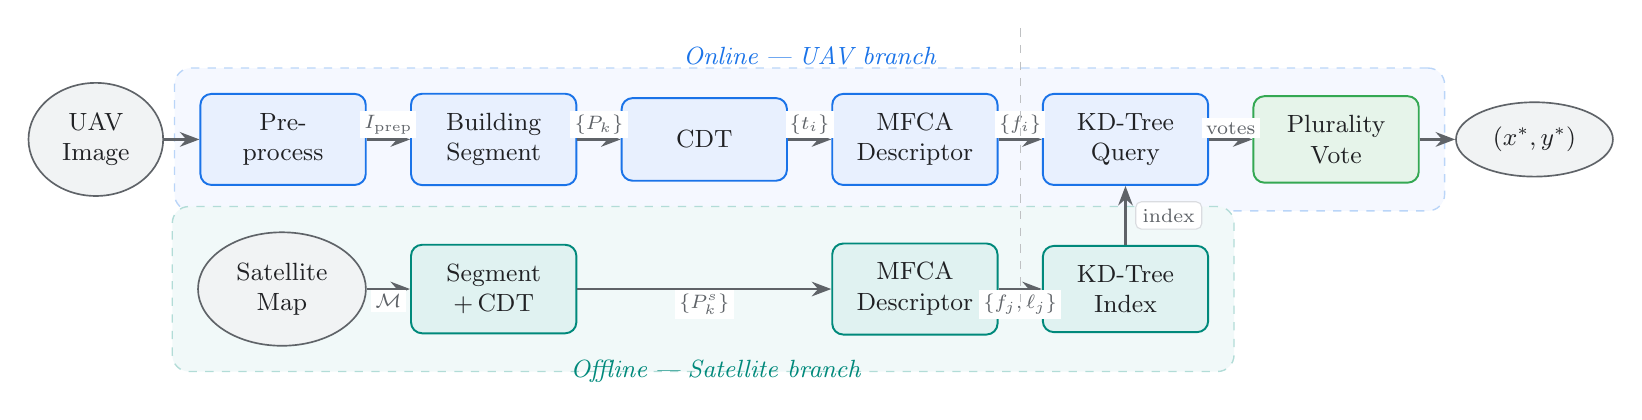
\begin{tikzpicture}[
  font=\small,
  base/.style  = {rounded corners=4pt, align=center, inner sep=7pt,
                  minimum width=2.10cm, minimum height=1.05cm,
                  line width=0.70pt, text=dmText},
  unode/.style = {base, fill=dmBlueL,  draw=dmBlue},
  snode/.style = {base, fill=dmTealL,  draw=dmTeal},
  onode/.style = {base, fill=dmGreenL, draw=dmGreen},
  term/.style  = {shape=ellipse, draw=dmGray, fill=dmGrayL, align=center,
                  inner sep=5pt, minimum width=1.42cm, minimum height=0.74cm,
                  line width=0.60pt, text=dmText},
  arr/.style   = {->, >=Stealth, line width=0.90pt, draw=dmGray},
  elbl/.style  = {font=\scriptsize, fill=white, inner sep=1.5pt,
                  text=dmGray, midway},
  bbox/.style  = {draw, dashed, rounded corners=6pt,
                  inner sep=9pt, line width=0.50pt},
]
 
%── Row 1: UAV branch (online) ───────────────────────────────────────────────
\node[term]  (ui)  {UAV\\Image};
\node[unode, right=0.45cm of ui]  (pre) {Pre-\\process};
\node[unode, right=0.55cm of pre] (seg) {Building\\Segment};
\node[unode, right=0.55cm of seg] (cdt) {CDT};
\node[unode, right=0.55cm of cdt] (des) {MFCA\\Descriptor};
\node[unode, right=0.55cm of des] (qry) {KD-Tree\\Query};
\node[onode, right=0.55cm of qry] (vot) {Plurality\\Vote};
\node[term,  right=0.45cm of vot] (pos) {$(x^*,y^*)$};
 
\draw[arr](ui)  -- (pre);
\draw[arr](pre) -- (seg) node[elbl,above]{$I_{\mathrm{prep}}$};
\draw[arr](seg) -- (cdt) node[elbl,above]{$\{P_k\}$};
\draw[arr](cdt) -- (des) node[elbl,above]{$\{t_i\}$};
\draw[arr](des) -- (qry) node[elbl,above]{$\{f_i\}$};
\draw[arr](qry) -- (vot) node[elbl,above]{votes};
\draw[arr](vot) -- (pos);
 
%── Row 2: Satellite branch (offline) ────────────────────────────────────────
%   sseg, sdes, sidx column-aligned under seg, des, qry respectively
\node[snode] (sseg) at ($(seg)+(0,-1.90)$) {Segment\\$+$\,CDT};
\node[term,  left=0.55cm of sseg] (si) {Satellite\\Map};
\node[snode] (sdes) at ($(des)+(0,-1.90)$) {MFCA\\Descriptor};
\node[snode] (sidx) at ($(qry)+(0,-1.90)$) {KD-Tree\\Index};
 
\draw[arr](si)   -- (sseg) node[elbl,below]{$\mathcal{M}$};
\draw[arr](sseg) -- (sdes) node[elbl,below]{$\{P_k^s\}$};
\draw[arr](sdes) -- (sidx) node[elbl,below]{$\{f_j,\ell_j\}$};
 
%── Cross-branch: offline index feeds online query ────────────────────────────
\draw[arr](sidx.north) -- (qry.south)
    node[midway, right=3.5pt, font=\scriptsize, fill=white,
         draw=dmGrayM, rounded corners=2pt, inner sep=2.5pt,
         text=dmGray, line width=0.40pt]{index};
 
%── Background panels ─────────────────────────────────────────────────────────
\begin{scope}[on background layer]
  \node[bbox, fill=dmBlueL!45, draw=dmBlue!30]  [fit=(pre)(vot)]  {};
  \node[bbox, fill=dmTealL!45, draw=dmTeal!30]  [fit=(si)(sidx)]  {};
\end{scope}
 
%── Offline / online divider ──────────────────────────────────────────────────
\coordinate (dv) at ($(des.north east)!0.5!(qry.north west)$);
\draw[dashed, dmGray!40, line width=0.50pt]
    ($(dv)+(0,+0.82)$) -- ($(dv)+(0,-2.74)$);
 
%── Branch labels ─────────────────────────────────────────────────────────────
\node[font=\small\itshape, text=dmBlue, above=7pt]
    at ($(pre.north west)!0.5!(vot.north east)$)
    {Online\;---\;UAV branch};
\node[font=\small\itshape, text=dmTeal, below=7pt]
    at ($(si.south west)!0.5!(sidx.south east)$)
    {Offline\;---\;Satellite branch};
 
\end{tikzpicture}%
}
\caption{%
  Two-branch localization pipeline.
  The \textit{online} UAV branch (blue) processes each query image through
  preprocessing, building segmentation, CDT, and MFCA descriptor
  extraction, then queries the pre-built KD-tree.
  The \textit{offline} satellite branch (teal) pre-computes descriptors
  and builds the KD-tree index once per map site; the dashed vertical
  line marks the offline/online boundary.
  Plurality voting over matched satellite triangles yields the predicted
  2-D position $(x^*,y^*)$.%
}
\label{fig:pipeline}
\end{figure}
\subsection{Building Polygon Decomposition via Constrained Delaunay Triangulation}
\label{sec:cdt}

\paragraph{Motivation.}
A polygon with $V$ vertices has no natural fixed-cardinality encoding, making
whole-polygon descriptors difficult to compare across buildings with differing
vertex counts.
Triangulation addresses this while delivering two additional properties.
First, \emph{matching density}: a building with $V$ vertices yields $V-2$
triangle descriptors via CDT, each an independent matching hypothesis.
A single building thus contributes up to $V-2$ votes to the patch estimator,
dramatically increasing robustness against individual false positives relative
to whole-polygon methods that produce a single vote per building.
Second, \emph{graceful degradation}: if segmentation merges two buildings into
one polygon, CDT still produces valid triangles from the merged shape, many of
which correctly match their satellite counterparts---a robustness property
that whole-polygon methods lack, since a merged polygon no longer resembles
either original building individually.

\paragraph{Definitions.}
Because every downstream stage operates on the triangles produced here, we
state the two notions explicitly rather than relying on citation alone. The
classical notion~\cite{delaunay1934} fixes only the empty-circle property; the
constrained variant~\cite{chew1989cdt} additionally forces a prescribed edge set.

\begin{definition}[Delaunay triangulation~\cite{delaunay1934}]
\label{def:dt}
Let $S\subset\mathbb{R}^2$ be a finite point set. A triangulation of (the convex
hull of) $S$ is a \emph{Delaunay triangulation} if it satisfies the
\emph{empty-circle property}: the circumscribed circle of every triangle
contains no point of $S$ in its interior. Equivalently, it lexicographically
maximises the sorted vector of triangle angles among all triangulations of $S$.
\end{definition}

\begin{definition}[Constrained Delaunay triangulation~\cite{chew1989cdt}]
\label{def:cdt}
Let $G=(S,E)$ be a planar straight-line graph on vertex set $S$ with a set of
prescribed (\emph{constrained}) edges $E$. A triangulation of $S$ is a
\emph{constrained Delaunay triangulation} (CDT) of $G$ if (i)~it contains every
edge of $E$, and (ii)~every other triangle satisfies the \emph{constrained}
empty-circle property: its circumcircle may contain a vertex of $S$ only if that
vertex is not visible from the triangle's interior, i.e.\ every segment to it
crosses some constrained edge. For a simple polygon $P_k$ we take $S$ to be its
vertices and $E$ its boundary edges~\eqref{eq:cdt_edges}, so the CDT triangulates
the polygon interior while keeping the building outline intact.
\end{definition}

\paragraph{Design.}
For each polygon $P_k$ with ordered vertices $v_1,\ldots,v_{V_k}$, the CDT of
Definition~\ref{def:cdt} is applied with the constrained edge set
\begin{equation}
E_{\mathrm{constrained}}^{(k)}
= \bigl\{(v_i,\,v_{i+1 \bmod V_k})\bigr\}_{i=1}^{V_k}
\label{eq:cdt_edges}
\end{equation}
consisting of all polygon boundary edges, which must appear in every CDT
of $P_k$ and prevent any interior edge from crossing the building boundary.
The constrained empty-circle condition then maximises minimum interior angles
within the edge-respecting family.
This produces a mesh $T^{(k)} = \{t_1,\ldots,t_{V_k-2}\}$ of
non-overlapping triangles (a simple polygon with $V_k$ vertices and no Steiner
points admits exactly $V_k-2$ triangles).

\begin{remark}[Uniqueness and its (non-)effect on our guarantees]
\label{rem:cdt_unique}
The (constrained) Delaunay triangulation of $P_k$ is \emph{unique} precisely
when its vertices are in \emph{general position}---no four mutually visible
vertices are cocircular~\cite{de1997computational}. Degenerate cocircular
configurations admit several equally valid CDTs. None of the properties we
invoke depends on uniqueness:
(i)~the triangle \emph{count} is triangulation-independent---any
Steiner-point-free triangulation of a simple $V_k$-gon has exactly $V_k-2$
triangles---so the matching-density argument and the $V_k-2$ votes per building
are unaffected;
(ii)~all Delaunay triangulations of a cocircular vertex group share the
\emph{same sorted angle vector} (equal subtended angles follow from the
inscribed-angle theorem), so the max--min angle optimality below is attained by
\emph{every} admissible CDT, and Propositions~\ref{prop:nondegen}--\ref{prop:sensitivity},
Theorem~\ref{thm:discriminative}, and Corollary~\ref{cor:separation}---all
stated per triangle---hold verbatim for whichever mesh is produced; and
(iii)~the implementation fixes a single deterministic tie-break (the
lexicographic vertex ordering used by \texttt{scipy.spatial}/\texttt{Triangle}),
so a given polygon always yields the same reproducible mesh, and the
plurality vote (Section~\ref{sec:vote}) aggregates over all $V_k-2$ triangles,
absorbing any residual per-triangle ambiguity.
\end{remark}

\paragraph{Technical advantage.}
Among all triangulations of $P_k$ that respect the constrained boundary edges,
CDT lexicographically maximizes the sorted vector of minimum
angles~\cite{de1997computational,chew1989cdt}; subject to the boundary
constraint it therefore avoids sliver triangles whose near-zero angles would
produce near-degenerate descriptors. (The classical max-min-angle optimality of
unconstrained Delaunay holds only over triangulations without forced edges; the
constrained variant attains the optimum within the admissible, edge-respecting
family.)

\subsection{MFCA Feature Extraction}
\label{sec:feat}
\label{sec:mfca}

\paragraph{Interior angle components.}
For triangle $t$ with vertices $v_A,v_B,v_C$, the three interior angles
$\alpha_A,\alpha_B,\alpha_C$ are computed analytically via the law of cosines.
The two smallest are selected and sorted:
$\alpha_1 \le \alpha_2$, both in $(0^\circ, 180^\circ)$.
These two components encode the \emph{shape} of the triangle independent of
position, orientation, or scale.

\paragraph{Ekeland's variational principle and its geometric instantiation.}
\label{para:ekeland}

The free-space component of our descriptor is \emph{inspired by}---not a
restatement of---Ekeland's variational principle.
From the principle we borrow one idea: a point is ``critical'' when a cone of
fixed slope can be brought up to touch a graph but cannot be pushed further
without crossing it.
We turn this idea into a concrete, computable quantity on building footprints,
the \textbf{Ekeland angle} $e_v$, whose per-triangle triplet is the Maximal Free
Cone Angle (MFCA).
We begin with the formal statement of the principle that motivates the
construction.

\begin{definition}[Ekeland's Variational Principle~\cite{ekeland1974}]
\label{def:ekeland}
Let $(\mathcal{X},d)$ be a complete metric space and
$\varphi: \mathcal{X} \to \mathbb{R} \cup \{+\infty\}$ be lower-semicontinuous
and bounded below.
For every $\varepsilon > 0$ and every $u \in \mathcal{X}$ with
$\varphi(u) \le \inf_{\mathcal{X}} \varphi + \varepsilon$, there exists
$\bar{x} \in \mathcal{X}$ satisfying:
\begin{enumerate}[label=(\roman*)]
  \item $\varphi(\bar{x}) \le \varphi(u)$ \hfill\emph{(improvement)}
  \item $d(\bar{x},u) \le 1$ \hfill\emph{(proximity)}
  \item $\varphi(\bar{x}) < \varphi(x) + \varepsilon \cdot d(\bar{x},x)$
        \;for all $x \ne \bar{x}$
        \hfill\emph{(strict cone criticality)}
\end{enumerate}
\end{definition}
\noindent(We write the abstract principle with $\varphi$ and $(\mathcal{X},d)$
to avoid collision with the descriptor $f$ and the triangle vertices used
throughout the rest of this section.)

Geometrically, condition (iii) says that no point $x \ne \bar{x}$ can improve
$\varphi$ beyond what the distance $d(\bar{x},x)$ ``pays for''.
Equivalently, the graph of $\varphi$ is touched from below at $\bar{x}$ by a
cone of slope $\varepsilon$ (the tent-shaped lower support in
Fig.~\ref{fig:ekeland_principle}), which cannot be raised without crossing the
graph.
This \emph{cone-touching} interpretation is the direct inspiration for the
Ekeland angle: we replace the abstract cone-on-a-graph with a concrete free
angular sector at a polygon vertex, and replace ``cannot be raised without
crossing the graph'' with ``cannot be widened without crossing a building
edge''.

\begin{figure}[htbp]
  \centering
  \resizebox{0.74\linewidth}{!}{%
  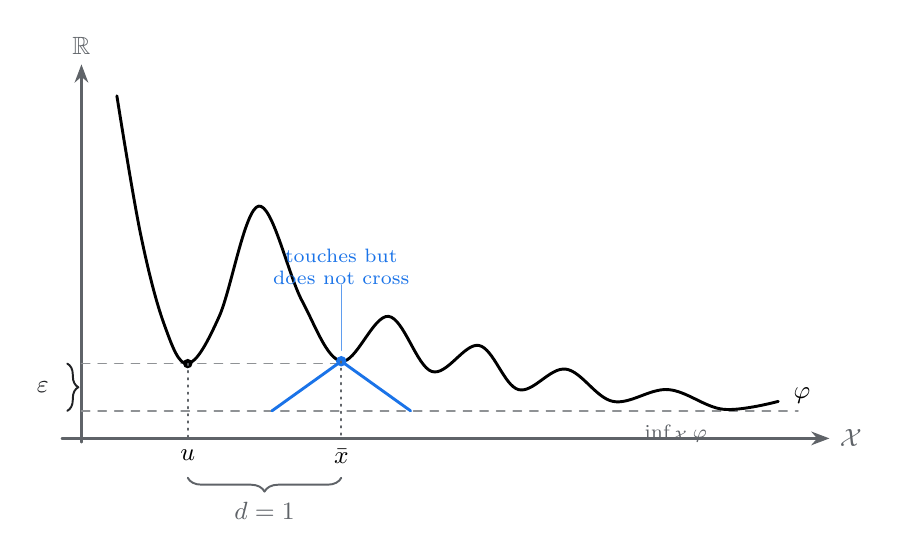
\begin{tikzpicture}[>=Stealth, line cap=round, line join=round, font=\small]
    % ── axes ──────────────────────────────────────────────────────────────
    \draw[dmGray, line width=0.8pt, ->] (0,-0.05) -- (0,4.75) node[above] {$\mathbb{R}$};
    \draw[dmGray, line width=0.8pt, ->] (-0.25,0) -- (9.5,0) node[right] {$\mathcal{X}$};

    % ── infimum baseline and inf+epsilon level (schematic) ─────────────────
    \draw[dmGray!70, dashed, line width=0.55pt] (0,0.35) -- (9.1,0.35);
    \node[dmGray, font=\scriptsize, anchor=north] at (7.55,0.30) {$\inf_{\mathcal{X}}\varphi$};
    \draw[dmGray!70, dashed, line width=0.55pt] (0,0.95) -- (3.3,0.95);
    % epsilon brace on the R axis between inf f and inf f + epsilon
    \draw[decorate, decoration={brace, amplitude=4pt}, dmText, line width=0.7pt]
      (-0.18,0.95) -- (-0.18,0.35) node[midway, left=3pt] {$\varepsilon$};

    % ── graph of f: lower-semicontinuous, bounded below, decaying ripples ──
    \draw[black, line width=1.05pt, smooth, tension=0.6]
      plot coordinates {
        (0.45,4.35) (0.75,2.60) (1.05,1.45) (1.35,0.95)
        (1.75,1.55) (2.25,2.95) (2.80,1.75) (3.30,0.98)
        (3.90,1.55) (4.45,0.85) (5.05,1.18) (5.55,0.62)
        (6.15,0.88) (6.75,0.47) (7.45,0.62) (8.15,0.37) (8.85,0.47)
      };
    \node[black] at (9.15,0.55) {$\varphi$};

    % ── u : an epsilon-approximate minimiser ──────────────────────────────
    \fill[black] (1.35,0.95) circle (1.7pt);
    \draw[dmGray, dotted, line width=0.6pt] (1.35,0.95) -- (1.35,0);
    \node[below] at (1.35,-0.02) {$u$};

    % ── v : the critical point, with the touching cone (slope epsilon) ─────
    \coordinate (V) at (3.30,0.98);
    % downward-opening tent y = f(v) - eps*|x-v|: a lower support touching at v
    \draw[dmBlue, line width=1.05pt] (V) -- (2.42,0.35);
    \draw[dmBlue, line width=1.05pt] (V) -- (4.18,0.35);
    \fill[dmBlue] (V) circle (1.9pt);
    \draw[dmGray, dotted, line width=0.6pt] (3.30,0.98) -- (3.30,0);
    \node[below] at (3.30,-0.02) {$\bar{x}$};
    \draw[dmBlue!70, line width=0.5pt] (3.30,1.95) -- (3.30,1.12);
    \node[dmBlue, font=\scriptsize, align=center] at (3.30,2.18)
      {touches but\\does not cross};

    % ── distance d = 1 between u and v ─────────────────────────────────────
    \draw[decorate, decoration={brace, amplitude=5pt, mirror}, dmGray, line width=0.7pt]
      (1.35,-0.50) -- (3.30,-0.50) node[midway, below=5pt] {$d = 1$};
  \end{tikzpicture}%
  }
  \caption{The classical Ekeland's variational principle
    (after Theorem~1 of~\cite{ekeland1974}), the inspiration for our descriptor.
    Starting from an $\varepsilon$-approximate minimiser $u$
    ($\varphi(u)\le\inf_{\mathcal{X}} \varphi+\varepsilon$), the principle yields
    a nearby point $\bar{x}$
    ($d(u,\bar{x})\le 1$) at which a cone of slope $\varepsilon$ (blue) touches the
    graph of $\varphi$ from below but cannot be pushed further without crossing it.
    We do not use the principle quantitatively; we borrow only this
    \emph{cone-touches-but-does-not-cross} criticality picture and instantiate
    it geometrically on building footprints, where the touching cone becomes
    the maximal free angular sector at a vertex (the Ekeland angle $e_v$) and
    the obstacle being touched is the boundary of the kernel expansion polygon
    $P_{\mathrm{sub}}$.}
  \label{fig:ekeland_principle}
\end{figure}

\smallskip
\noindent\textit{Structural instantiation in the UAV plane.}
Unlike abstract metric-space formulations that apply the principle
rhetorically, our construction instantiates Ekeland's principle
\emph{structurally}: every element of the principle corresponds to a concrete,
computable geometric object.

\begin{itemize}[leftmargin=*,topsep=2pt]
  \item \textbf{Complete metric space $(\mathcal{X},d)$:}
        $(\partial P_{\mathrm{sub}},\, d_{\mathrm{arc}})$---the boundary of
        the kernel polygon $P_{\mathrm{sub}}$ with arc-length metric.
  \item \textbf{Function $\varphi$ bounded below:}
        $g(\hat{b}) = -\Theta(X,\hat{b})$, where
        $\Theta(X,\hat{b})$ is the angular width of the largest obstacle-free
        sector at vertex $X$ that contains direction $\hat{b}$ and whose
        interior avoids $\partial P_{\mathrm{sub}}$.
        $g$ is lower-semicontinuous (blockage events are closed) and bounded
        below by $-360^\circ$; its \emph{unconstrained} maximal free width equals
        the exterior angle $\alpha(X)$.
  \item \textbf{Axis-anchored critical cone:}
        the reference ray $X\mathbf{d}\parallel O_x/O_y$ is the (constrained)
        cone axis; the cone symmetric about $X\mathbf{d}$ grows until a bounding
        ray meets the nearer incident edge, which then lies \emph{tangent to
        $\partial P_{\mathrm{sub}}$}---it touches but does not cross the obstacle,
        exactly as Ekeland's cone touches but does not cross the graph of
        $\varphi$ (Definition~\ref{def:ekeland}(iii)). The unconstrained optimum
        is the wedge bisector (value $\alpha(X)$); the axis constraint gives
        $e_X\le\alpha(X)$, equality iff $X\mathbf{d}$ bisects the wedge.
  \item \textbf{Stopping criterion = criticality condition:}
        $P_{\mathrm{sub}}$ is the \emph{largest} polygon obtained by merging
        adjacent CDT triangles such that all three original triangle vertices
        $v_A,v_B,v_C$ remain on $\partial P_{\mathrm{sub}}$ with exterior wedge
        ${>}90^\circ$.
        This is the Ekeland critical-point condition: $P_{\mathrm{sub}}$
        cannot be expanded further while keeping the triangle vertices as
        boundary (critical) points with a well-defined touching cone---any
        further merge would either push a vertex into the interior (destroying
        criticality) or collapse its wedge below the function condition
        (Fig.~\ref{fig:spike}).
  \item \textbf{Ekeland angle $e_v$:}
        $e_v=\min(\angle\mathbf{a}v\mathbf{a}',\,\angle\mathbf{b}v\mathbf{b}')
        =2\min(\theta_a,\theta_b)$, capped at $180^\circ$ for convex $v$---the
        width of the axis-anchored touching cone, the analogue of the critical
        value $\varphi(\bar{x})$.
\end{itemize}

Table~\ref{tab:ekeland_correspondence} displays the complete correspondence.

\begin{table}[h]
\caption{Structural correspondence between Ekeland's variational principle
         and the edge-anchored Ekeland angle (this work).}
\label{tab:ekeland_correspondence}
\centering\small
\begin{tabular}{p{5.2cm}p{7.8cm}}
\toprule
\textbf{Ekeland's Principle} & \textbf{Ekeland Angle — this work} \\
\midrule
Complete metric space $(\mathcal{X},d)$
  & $(\partial P_{\mathrm{sub}},\,d_{\mathrm{arc}})$: polygon boundary,
    arc-length \\
Function $\varphi$ bounded below
  & $g(\hat{b}) = {-}\Theta(X,\hat{b})$: negated free-sector width \\
$\varepsilon$-cone of slope $\varepsilon$
  & Cone symmetric about axis ray $X\mathbf{d}\parallel O_x/O_y$ at vertex $X$ \\
Cone \emph{touches but does not cross} $\varphi$
  & Bounding ray tangent to the nearer $\partial P_{\mathrm{sub}}$ edge \\
Stopping = criticality condition
  & Merge halts when a vertex would leave $\partial P_{\mathrm{sub}}$ or its wedge would drop below $90^\circ$ \\
Value $\varphi(\bar{x})$ at critical point
  & $e_X = \min(\angle\mathbf{a}X\mathbf{a}',\angle\mathbf{b}X\mathbf{b}')=2\min(\theta_a,\theta_b)$, capped at $180^\circ$ \\
Stability: no free gain without distance cost
  & No cone enlargement without crossing an obstacle edge \\
Unconstrained optimum ($\varepsilon\to0$)
  & $e_X=\alpha(X)$ iff $X\mathbf{d}$ bisects the wedge; in general $e_X\le\alpha(X)$, exact and $O(1)$ \\
\bottomrule
\end{tabular}
\end{table}

\paragraph{Why we expand: the kernel expansion as a non-degeneracy device.}
The Ekeland angle alone, read off a \emph{bare} CDT triangle, is uninformative:
the three interior angles of any triangle are each below $180^\circ$ (every
corner is a convex vertex of the triangle as a polygon), so the exterior angle
$\alpha(X)=360^\circ-\alpha_{\mathrm{int}}(X)$---where $\alpha_{\mathrm{int}}(X)$
is the interior angle of $P_{\mathrm{sub}}$ at $X$ (Table~\ref{tab:notation})---exceeds $180^\circ$ at all three
vertices, which is the convex case, so $e_X$ saturates at $180^\circ$.
A descriptor built from bare triangles would therefore saturate its entire
free-space sub-vector at $(180^\circ,180^\circ,180^\circ)$, carrying no
within-building shape-context information.
The \emph{kernel expansion} $P_{\mathrm{sub}}$ is our proposed remedy: by
merging neighbouring triangles under the boundary-preserving stopping rule, it
reshapes the local neighbourhood of each seed vertex so that the resulting
Ekeland angles avoid the two degenerate extremes of the $(0^\circ,180^\circ]$
range.
We state the resulting guarantees first and give the explicit construction
afterwards; the propositions below use only two facts, made precise in
Definition~\ref{def:ekeland_angle} and Eq.~\eqref{eq:ekeland_bound}: $e_X=180^\circ$
at a convex vertex, and $0^\circ<e_X\le360^\circ-\alpha_{\mathrm{int}}(X)<180^\circ$
at a reflex vertex (the lower bound guaranteed by the $90^\circ$ wedge guard,
Lemma~\ref{lem:axis_exists}).
Proposition~\ref{prop:nondegen} makes both effects precise: expansion (1)~keeps
every Ekeland angle \emph{strictly above} $0^\circ$, and (2)~drives angles
\emph{below} the saturated $180^\circ$ wherever the surrounding geometry is
non-trivial.
Together these push the descriptor distribution away from $\{0^\circ,180^\circ\}$
and into the informative interior, which is exactly where $\ell_1$ matching
discriminates.

\begin{proposition}[Non-degeneracy under kernel expansion]
\label{prop:nondegen}
Let $X\in\{v_A,v_B,v_C\}$ be a seed-triangle vertex and let $P_{\mathrm{sub}}$
be its kernel expansion polygon obtained by Algorithm~\ref{alg:mfca} (Phase~1).
Then:
\begin{enumerate}[label=(\arabic*)]
  \item \textbf{No $0^\circ$ values.}
        $e_X(P_{\mathrm{sub}}) > 0^\circ$.
        Equivalently, no seed vertex is ever assigned a vanishing free angle.
  \item \textbf{Reduced $180^\circ$ values.}
        Let $e_X^{0}=180^\circ$ be the Ekeland angle of the bare seed triangle.
        Then $e_X(P_{\mathrm{sub}}) \le e_X^{0}$, with strict inequality
        $e_X(P_{\mathrm{sub}}) < 180^\circ$ whenever expansion makes $X$ a reflex
        vertex of $P_{\mathrm{sub}}$ (i.e.\ $\alpha_{\mathrm{int}}(X) > 180^\circ$).
        Consequently the number of saturated ($180^\circ$) components of the
        MFCA triplet is non-increasing under expansion and strictly decreasing
        at every seed vertex that becomes reflex.
\end{enumerate}
\end{proposition}
\begin{proof}
By the Phase-1 guard every seed vertex has $\alpha_{\mathrm{int}}(X)<270^\circ$,
so its exterior wedge has width $\alpha(X)=360^\circ-\alpha_{\mathrm{int}}(X)>90^\circ$,
and Lemma~\ref{lem:axis_exists} provides an axis ray $X\mathbf{d}$ strictly inside
it, i.e.\ $\theta_a,\theta_b>0$.

(1) In the convex case $e_X=180^\circ>0^\circ$. In the reflex case
$e_X=2\min(\theta_a,\theta_b)>0^\circ$ because $\theta_a,\theta_b>0$. A vanishing
value $e_X=0^\circ$ would force $X$ into the interior of $P_{\mathrm{sub}}$
($\alpha_{\mathrm{int}}(X)=360^\circ$), which the stopping rule forbids.

(2) The bare seed triangle is convex at every vertex
($\alpha_{\mathrm{int}}(X)<180^\circ$), so $e_X^{0}=180^\circ$. After expansion,
either $X$ is still convex and $e_X=180^\circ$, or $X$ is reflex and, by
Eq.~\eqref{eq:ekeland_bound},
$e_X\le\alpha(X)=360^\circ-\alpha_{\mathrm{int}}(X)<180^\circ$.
Hence $e_X(P_{\mathrm{sub}})\le e_X^{0}=180^\circ$, with strict inequality
exactly when expansion makes $X$ reflex. The count statement follows
vertexwise. \qed
\end{proof}

\begin{remark}
Proposition~\ref{prop:nondegen} is the formal justification for proposing the
kernel expansion at all.
Without it the MFCA collapses to the constant $180^\circ$; with it the MFCA
becomes a genuine, bounded, non-degenerate signal in $(0^\circ,180^\circ]$
whose value reports how enclosed each vertex is by the surrounding building
geometry.
This is what makes two same-shape triangles in different urban contexts
separable in $\ell_1$ (Corollary~\ref{cor:separation}).
\end{remark}

\paragraph{Mathematical properties.}

We now establish further formal properties of the Ekeland angle that justify
its use as a discriminative descriptor component.

\begin{proposition}[Monotone envelope under kernel expansion]
\label{prop:monotone}
Let $P_{\mathrm{sub}} \subseteq P'_{\mathrm{sub}}$ be two kernel expansions at
vertex $X$ ($P'_{\mathrm{sub}}$ merges additional triangles). Then the exterior
angle (the cap on $e_X$) is non-increasing,
\[
  \alpha(X;P_{\mathrm{sub}})\;\ge\;\alpha(X;P'_{\mathrm{sub}}),
  \qquad e_X\le\alpha(X)\ \text{in both (Eq.~\eqref{eq:ekeland_bound}),}
\]
so expansion can only tighten the admissible range of $e_X$ downward.
In particular, if $X$ is convex in $P_{\mathrm{sub}}$ ($e_X=180^\circ$) and
reflex in $P'_{\mathrm{sub}}$, then
$e_X(P'_{\mathrm{sub}})<180^\circ=e_X(P_{\mathrm{sub}})$.
\end{proposition}
\begin{proof}
Merging triangles at $X$ never decreases the interior angle
$\alpha_{\mathrm{int}}(X)$---a merge either preserves the local boundary at $X$
or enlarges the interior---so $\alpha(X)=360^\circ-\alpha_{\mathrm{int}}(X)$ is
non-increasing. The bound $e_X\le\alpha(X)$ is Eq.~\eqref{eq:ekeland_bound}
(in the convex case $e_X=180^\circ\le\alpha(X)$). The convex-to-reflex drop is
Proposition~\ref{prop:nondegen}(2). \qed
\end{proof}

\begin{remark}
The cap $\alpha(X)$ and the convex$\to$reflex transition are monotone, but the
\emph{pointwise} value $e_X=2\min(\theta_a,\theta_b)$ need not be: the incident
edge directions---hence $\theta_a,\theta_b$---change as different triangles are
merged, so $e_X$ can fluctuate within $(0^\circ,\alpha(X)]$. Under a fixed local
orientation (the axis ray keeping the same relation to the two edges) the value
itself is monotone. The design intent is unchanged: vertices in complex building
recesses (reflex, small $\alpha(X)$) are confined to small Ekeland angles, while
isolated corners stay at $e_X=180^\circ$.
\end{remark}

\begin{proposition}[Exterior-angle bound and tightness]
\label{prop:sensitivity}
Let $X$ be a reflex seed vertex, so (by the Phase-1 guard)
$90^\circ<\alpha(X)<180^\circ$. With $\theta_a,\theta_b$ the angles from the
reference ray $X\mathbf{d}$ to the two incident edges
($\theta_a+\theta_b=\alpha(X)$),
\begin{equation}
  e_X \;=\; 2\min(\theta_a,\theta_b)
       \;\in\;(0^\circ,\,\alpha(X)],
  \qquad
  e_X \;\le\; \alpha(X) \;=\; 360^\circ-\alpha_{\mathrm{int}}(X),
\label{eq:sensitivity_bound}
\end{equation}
with equality $e_X=\alpha(X)$ iff $X\mathbf{d}$ bisects the wedge
($\theta_a=\theta_b$). Consequently $e_X$ is monotone non-increasing in
$\alpha_{\mathrm{int}}(X)$ at fixed orientation, and strictly below the
convex value $180^\circ$ whenever $X$ is reflex.
\end{proposition}
\begin{proof}
Reflecting the incident edges across $X\mathbf{d}$ gives
$\angle\mathbf{a}X\mathbf{a}'=2\theta_a$ and $\angle\mathbf{b}X\mathbf{b}'=2\theta_b$
(Eq.~\eqref{eq:ekeland_bound}); the definition takes the minimum, so
$e_X=2\min(\theta_a,\theta_b)$. Since $\min(\theta_a,\theta_b)\le(\theta_a+\theta_b)/2$,
we get $e_X\le\theta_a+\theta_b=\alpha(X)$, with equality iff
$\theta_a=\theta_b$. As $\theta_a,\theta_b>0$ (Lemma~\ref{lem:axis_exists}),
$e_X>0^\circ$; and $\alpha(X)<180^\circ$ for reflex $X$ gives $e_X<180^\circ$.
\qed
\end{proof}

\begin{theorem}[Discriminativeness of the 5-D descriptor]
\label{thm:discriminative}
Let $f^t = (\alpha_1^t, \alpha_2^t, e_1^t, e_2^t, e_3^t)$ and
$f^{t'} = (\alpha_1^{t'}, \alpha_2^{t'}, e_1^{t'}, e_2^{t'}, e_3^{t'})$
be the 5-D descriptors of triangles $t$ and $t'$, where
$(\alpha_1,\alpha_2)$ is the sorted shape pair and $(e_1\le e_2\le e_3)$ is the
sorted Ekeland triplet (the MFCA, Table~\ref{tab:notation}).
Then $f^t \ne f^{t'}$ if and only if either:
\begin{enumerate}[label=(\alph*)]
  \item the triangles have different shapes:
        $(\alpha_1^t, \alpha_2^t) \ne (\alpha_1^{t'}, \alpha_2^{t'})$, or
  \item the sorted Ekeland triplets differ:
        $(e_1^t, e_2^t, e_3^t) \ne (e_1^{t'}, e_2^{t'}, e_3^{t'})$.
\end{enumerate}
Moreover, if condition (a) fails (equal shapes) but at least one sorted Ekeland
angle differs by $\Delta > 0$, then:
\begin{equation}
  \|f^t - f^{t'}\|_1 \;\ge\; \Delta.
\label{eq:descriptor_lb}
\end{equation}
\end{theorem}
\begin{proof}
The first claim follows directly from the coordinate definition
$f = (\alpha_1,\alpha_2,e_1,e_2,e_3)$: $f^t \ne f^{t'}$ iff at least one
coordinate differs, which is exactly the disjunction of (a) and (b).

For the bound: suppose $(\alpha_1^t,\alpha_2^t) = (\alpha_1^{t'},\alpha_2^{t'})$
and $e_i^t \ne e_i^{t'}$ for some $i \in \{1,2,3\}$ with $|e_i^t - e_i^{t'}|
\ge \Delta$.
Then
\begin{align*}
  \|f^t - f^{t'}\|_1
  &= \underbrace{|\alpha_1^t - \alpha_1^{t'}|}_{=0}
   + \underbrace{|\alpha_2^t - \alpha_2^{t'}|}_{=0}
   + \sum_{j=1}^{3}|e_j^t - e_j^{t'}|
  \;\ge\; |e_i^t - e_i^{t'}| \;\ge\; \Delta.
\end{align*}
\end{proof}

\begin{corollary}[Shape-context separation]
\label{cor:separation}
Let two triangles have identical shape $(\alpha_1,\alpha_2)$ but kernel
expansions that differ in enclosure, so that some sorted Ekeland angle differs
by $\Delta=|e_{(i)}^t-e_{(i)}^{t'}|>0$. Then
\begin{equation}
  \|f^t - f^{t'}\|_1 \;\ge\; \Delta,
\end{equation}
whereas the pure interior-angle descriptor $(\alpha_1,\alpha_2)$ has $\ell_1$
distance \emph{zero} between them.
\end{corollary}
\begin{proof}
Equal shapes give $|\alpha_1^t-\alpha_1^{t'}|=|\alpha_2^t-\alpha_2^{t'}|=0$, so
$\|f^t-f^{t'}\|_1=\sum_{j=1}^3|e_{(j)}^t-e_{(j)}^{t'}|\ge|e_{(i)}^t-e_{(i)}^{t'}|=\Delta$.
The shape-only distance is $0$ by assumption. \qed
\end{proof}

Corollary~\ref{cor:separation} is the formal statement of the
building-recess vs.\ isolated-corner intuition: two same-shape triangles whose
kernel polygons enclose their shared vertex differently produce different
Ekeland angles, hence nonzero $\ell_1$ separation, while the shape-only
descriptor cannot tell them apart. By Proposition~\ref{prop:sensitivity} each
reflex vertex contributes $e_X\le 360^\circ-\alpha_{\mathrm{int}}(X)$, so the
gap can be as large as $180^\circ$ at the extreme of a deep recess
($e_X\!\to\!0^\circ$) versus a fully convex isolated corner ($e_X=180^\circ$).


\paragraph{Motivation.}
Interior angles alone are insufficient to discriminate triangles sitting in
different within-building shape contexts.
Consider a right-angle building corner in two locations: one at an isolated
building (all adjacent CDT triangles merge readily into $P_{\mathrm{sub}}$,
keeping the vertex convex), the other at a concave building recess (merging
adjacent triangles creates a reflex configuration at the original vertex).
Both corners may share identical interior-angle sub-vectors
$(\alpha_1 = 45^\circ, \alpha_2 = 45^\circ)$.
The Ekeland angle discriminates them: the convex vertex (exterior angle
$\alpha(v) \ge 180^\circ$) yields $e_v = 180^\circ$ (exterior free space is wide),
while the reflex vertex (exterior angle $90^\circ<\alpha(v) < 180^\circ$) yields
$0^\circ<e_v \le \alpha(v) = 360^\circ - \alpha_{\mathrm{int}}(v) < 180^\circ$ via
the axis-anchored reflection (exterior free space is compressed).
The discrimination is encoded directly in the shape of $P_{\mathrm{sub}}$:
the maximal expansion polygon whose stopping criterion (all three original
vertices stay on the boundary with wedge ${>}90^\circ$) is the Ekeland
criticality condition with its function hypothesis.

\paragraph{Obstacle set.}
The obstacle for the Ekeland angle computation at each vertex $v$ is
\emph{solely the boundary of $P_{\mathrm{sub}}$}:
\begin{equation}
  \mathcal{O}_v \;=\; \partial P_{\mathrm{sub}}
  \;=\; \{\text{boundary edges of the kernel expansion polygon } P_{\mathrm{sub}}\}.
  \label{eq:obstacle}
\end{equation}
This is geometrically motivated: $P_{\mathrm{sub}}$ is the maximal polygon
whose stopping condition instantiates Ekeland's criticality---its boundary is
therefore the tightest obstacle that the principle's cone can touch without
crossing.
No external neighbor polygon set or search radius $r$ is required.

\paragraph{Edge-anchored definition.}
Let $X \in \{v_A,v_B,v_C\}$ be a seed vertex on $\partial P_{\mathrm{sub}}$, with
incident boundary edges $\mathbf{a}$ (toward $X_{\mathrm{prev}}$) and $\mathbf{b}$
(toward $X_{\mathrm{next}}$). Let $\alpha_{\mathrm{int}}(X)$ be the interior angle
of $P_{\mathrm{sub}}$ at $X$ and $\alpha(X)=360^\circ-\alpha_{\mathrm{int}}(X)$
the exterior angle---the angular width of the free wedge $\angle\mathbf{a}X\mathbf{b}$
\emph{outside} $P_{\mathrm{sub}}$, which is the obstacle the Ekeland cone must
touch but not cross.

\begin{definition}[Ekeland Angle at vertex $X$]
\label{def:ekeland_angle}
\leavevmode
\begin{itemize}[leftmargin=*,topsep=2pt]
\item \emph{Convex case} ($\alpha(X)\ge180^\circ$, i.e.\ $\alpha_{\mathrm{int}}(X)\le180^\circ$):
      the free exterior wedge is at least a half-plane, the touching cone is
      unobstructed, and we set $e_X = 180^\circ$.
\item \emph{Reflex case} ($\alpha(X)<180^\circ$, i.e.\ $\alpha_{\mathrm{int}}(X)>180^\circ$):
      take a reference ray $X\mathbf{d}$ from $X$ parallel to the $O_x$ or $O_y$
      axis and lying inside the free wedge $\angle\mathbf{a}X\mathbf{b}$ (it
      exists by Lemma~\ref{lem:axis_exists}). Reflect the incident edge
      directions $\hat{\mathbf{a}},\hat{\mathbf{b}}$ across $X\mathbf{d}$ to get
      $\hat{\mathbf{a}}',\hat{\mathbf{b}}'$, and set
      \begin{equation}
        e_X \;=\; \min\bigl(\,\angle\mathbf{a}X\mathbf{a}',\ \angle\mathbf{b}X\mathbf{b}'\,\bigr).
        \label{eq:ekeland_angle}
      \end{equation}
\end{itemize}
\end{definition}

\noindent\emph{Reading as Ekeland's touching cone.}
The reference ray $X\mathbf{d}$ plays the role of the \emph{cone axis}, and the
reflection builds the widest cone \emph{symmetric about $X\mathbf{d}$} whose two
bounding rays do not cross $\partial P_{\mathrm{sub}}$: reflecting an incident
edge across the axis gives the half-cone on that side, and the binding (nearer)
edge fixes the half-width. This is precisely Ekeland's
``cone touches but does not cross'' picture (Definition~\ref{def:ekeland},
condition~(iii)), with the cone here constrained to be centred on an
axis-parallel ray. Writing $\theta_a,\theta_b$ for the angles from $X\mathbf{d}$
to $\mathbf{a},\mathbf{b}$ (so $\theta_a+\theta_b=\alpha(X)$), the reflected
angles are $\angle\mathbf{a}X\mathbf{a}'=2\theta_a$ and
$\angle\mathbf{b}X\mathbf{b}'=2\theta_b$, hence
\begin{equation}
  e_X \;=\; 2\min(\theta_a,\theta_b)\;\le\;\theta_a+\theta_b\;=\;\alpha(X)
          \;=\;360^\circ-\alpha_{\mathrm{int}}(X),
  \label{eq:ekeland_bound}
\end{equation}
with equality iff $\theta_a=\theta_b$, i.e.\ iff the forced axis $X\mathbf{d}$
happens to bisect the wedge---the direction the \emph{unconstrained} Ekeland cone
of Definition~\ref{def:ekeland} would select. Thus $e_X$ is a tight,
axis-aligned realisation of the exterior angle, never exceeding it.
The construction is \textbf{exact} (no angular sweep) and \textbf{$O(1)$ per
vertex}: by Eq.~\eqref{eq:ekeland_bound} one need only identify the nearer edge,
read off in a single test---whichever reflected ray overshoots the opposite edge
marks the \emph{farther} edge, so the \emph{other} reflected angle is $e_X$ (if
$\hat{\mathbf a}'$ crosses $\mathbf{b}$ then $e_X=\angle\mathbf{b}X\mathbf{b}'$,
and symmetrically). The axis-parallel choice makes $e_X$ meaningful for the
downstream \emph{axis-aligned} (north-up) localization task; $e_X$ is not
rotation-invariant on its own, but query and map are yaw-aligned to a common
north-up frame (Step~1b, Section~\ref{sec:preproc}), so both descriptors are
computed in the same axes (cf.\ the invariance discussion in
Section~\ref{sec:intro}).

\paragraph{Existence of the cone and the function condition.}
In Ekeland's principle the touching cone is guaranteed because $\varphi$ is a
\emph{function}: over the domain there is a single graph for the cone to meet.
The geometric analogue can fail. At a thin spike (Fig.~\ref{fig:spike}) the
boundary near $X$ is not single-valued over either axis and no axis-parallel ray
fits inside the (now sub-$90^\circ$) wedge, so no symmetric touching cone---hence
no Ekeland angle---exists there, exactly the configuration Ekeland's function
hypothesis excludes. We rule this out at the source through the kernel-expansion
stopping rule (Algorithm~\ref{alg:mfca}, Phase~1), which keeps every seed
vertex's exterior wedge wider than $90^\circ$:

\begin{lemma}[Axis reference ray exists]
\label{lem:axis_exists}
If the free exterior wedge at $X$ has width $\alpha(X)>90^\circ$, it contains at
least one of the four axis half-rays $\{+O_x,-O_x,+O_y,-O_y\}$; that direction is
interior to the open wedge, so the ray $X\mathbf{d}$ of
Definition~\ref{def:ekeland_angle} exists and lies strictly inside the wedge.
\end{lemma}
\begin{proof}
The four axis half-ray directions are equally spaced $90^\circ$ apart. Two
consecutive directions bound an open gap of width exactly $90^\circ$; an open
angular interval of width ${>}90^\circ$ cannot fit inside such a gap, hence
contains at least one axis direction. \qed
\end{proof}

\noindent Because Phase~1 enforces $\alpha_{\mathrm{int}}(X)<270^\circ$ at every
seed vertex, the reflex case always has
$\alpha(X)=360^\circ-\alpha_{\mathrm{int}}(X)>90^\circ$, so by
Lemma~\ref{lem:axis_exists} the ray $X\mathbf{d}$ exists, $\theta_a,\theta_b>0$,
and $e_X$ is always well defined in $(0^\circ,180^\circ]$. The degenerate spike
of Fig.~\ref{fig:spike} never arises in $P_{\mathrm{sub}}$.

\begin{figure}[htbp]
  \centering
  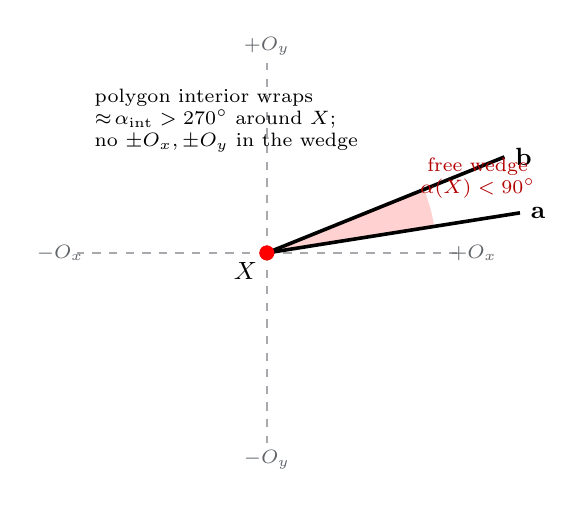
\begin{tikzpicture}[>=Stealth,scale=1.05,line join=round,font=\small]
    \coordinate (X) at (0,0);
    % candidate axis half-ray directions from X
    \foreach \a in {0,90,180,270}
       \draw[dmGray!55,dashed,line width=0.5pt] (X) -- (\a:2.3);
    \node[dmGray,font=\scriptsize] at (2.5,0) {$+O_x$};
    \node[dmGray,font=\scriptsize] at (0,2.5) {$+O_y$};
    \node[dmGray,font=\scriptsize] at (-2.5,0) {$-O_x$};
    \node[dmGray,font=\scriptsize] at (0,-2.5) {$-O_y$};
    % thin exterior free wedge between edges a (9 deg) and b (22 deg)
    \fill[red!18] (X) -- (9:2.05) arc[start angle=9,end angle=22,radius=2.05] -- cycle;
    % incident edges (nearly parallel -> narrow exterior wedge; interior is the rest)
    \draw[line width=1.3pt] (X) -- (9:3.1)  node[right]{$\mathbf{a}$};
    \draw[line width=1.3pt] (X) -- (22:3.1) node[right]{$\mathbf{b}$};
    \fill[red] (X) circle (2.6pt);
    \node[below left] at (X) {$X$};
    \node[align=center,font=\scriptsize,red!70!black] at (2.55,0.9)
       {free wedge\\$\alpha(X)<90^\circ$};
    \node[align=left,font=\scriptsize,anchor=west] at (-2.2,1.6)
       {polygon interior wraps\\$\approx\!\alpha_{\mathrm{int}}>270^\circ$ around $X$;\\
        no $\pm O_x,\pm O_y$ in the wedge};
  \end{tikzpicture}
  \caption{Degenerate thin spike excluded by the Phase-1 guard
    $\alpha_{\mathrm{int}}(X)<270^\circ$. The two incident edges
    $\mathbf{a},\mathbf{b}$ are nearly parallel, so the free exterior wedge
    $\alpha(X)<90^\circ$ contains none of the four axis half-rays: no symmetric
    cone can be anchored, and---mirroring Ekeland's requirement that $\varphi$ be
    a function---no Ekeland angle exists at $X$.}
  \label{fig:spike}
\end{figure}


\paragraph{Algorithm.}

\begin{algorithm}[htbp]
\caption{Axis-Parallel Reflection Ekeland Angle at triangle vertices}
\label{alg:mfca}
\begin{algorithmic}[1]
\Require Triangle $T=(v_A,v_B,v_C) \in P_k$, CDT mesh $\mathcal{T}^{(k)}$,
         max depth $D_{\max}$
\Ensure $(e_{v_A},\,e_{v_B},\,e_{v_C})$

\smallskip
\State \textbf{--- Phase 1: Ekeland Kernel Expansion (build $P_{\mathrm{sub}}$) ---}
\State $P_{\mathrm{sub}} \leftarrow T$;\quad $\mathrm{depth} \leftarrow 0$
\Repeat
  \State $\mathrm{merged} \leftarrow \mathtt{false}$
  \For{each $t'$ sharing an edge with $P_{\mathrm{sub}}$, $t' \in \mathcal{T}^{(k)}$}
    \State $P' \leftarrow P_{\mathrm{sub}} \cup t'$ \quad\Comment{tentative merge}
    \If{$v_A,v_B,v_C$ all remain on $\partial P'$ \textbf{and}
        $\alpha_{\mathrm{int}}(v_A),\alpha_{\mathrm{int}}(v_B),\alpha_{\mathrm{int}}(v_C)<270^\circ$ in $P'$}
      \State $P_{\mathrm{sub}} \leftarrow P'$;\quad
             $\mathrm{merged} \leftarrow \mathtt{true}$;\quad \textbf{break}
             \Comment{guard keeps each wedge $\alpha(v_\bullet)>90^\circ$}
    \EndIf
  \EndFor
  \State $\mathrm{depth} \mathrel{+}= 1$
\Until{$\lnot\,\mathrm{merged}$ \textbf{or} $\mathrm{depth} = D_{\max}$}
\Comment{Invariant: $v_A,v_B,v_C \in \partial P_{\mathrm{sub}}$, $\alpha_{\mathrm{int}}(\cdot)<270^\circ$}

\smallskip
\State \textbf{--- Phase 2: Axis-Parallel Reflection Ekeland Angle ---}
\For{each $X \in \{v_A,v_B,v_C\}$}
  \State $\mathbf{a},\mathbf{b} \leftarrow$ the two $\partial P_{\mathrm{sub}}$ edges incident to $X$
         (toward $X_{\mathrm{prev}},X_{\mathrm{next}}$)
  \State $\alpha(X) \leftarrow 360^\circ - \alpha_{\mathrm{int}}(X)$
         \Comment{exterior wedge width $\angle\mathbf{a}X\mathbf{b}$}
  \If{$\alpha(X) \ge 180^\circ$} \Comment{convex vertex: free exterior space $\ge$ half-plane}
    \State $e_X \leftarrow 180^\circ$
  \Else \Comment{reflex vertex: $90^\circ<\alpha(X)<180^\circ$ by Phase-1 guard}
    \State choose $X\mathbf{d}\parallel O_x$ or $O_y$ inside the wedge $\angle\mathbf{a}X\mathbf{b}$
           \Comment{exists, Lemma~\ref{lem:axis_exists}}
    \State reflect $\hat{\mathbf{a}},\hat{\mathbf{b}}$ across $X\mathbf{d}$ to get $\hat{\mathbf{a}}',\hat{\mathbf{b}}'$
    \State $e_X \leftarrow \min\bigl(\angle\mathbf{a}X\mathbf{a}',\,\angle\mathbf{b}X\mathbf{b}'\bigr)$
           \Comment{$=2\min(\theta_a,\theta_b)\le\alpha(X)$, Eq.~\eqref{eq:ekeland_bound}}
  \EndIf
\EndFor
\Return $(e_{v_A},\,e_{v_B},\,e_{v_C})$
\end{algorithmic}
\end{algorithm}

\noindent\textbf{Correctness of Phase 1 (termination and invariant).}
Each iteration merges at most one triangle; $|\mathcal{T}^{(k)}|$ is finite;
therefore Phase 1 halts in at most $\min(|\mathcal{T}^{(k)}|, D_{\max})$
iterations.
The invariant
$v_A,v_B,v_C \in \partial P_{\mathrm{sub}}$ with $\alpha_{\mathrm{int}}(\cdot)<270^\circ$
is maintained by construction: a merge is accepted only if all three seed
vertices stay on the boundary \emph{and} keep their exterior wedge wider than
$90^\circ$ (Lemma~\ref{lem:axis_exists}).
The stopping condition is the direct Ekeland criticality condition: when
no merge can be accepted, $P_{\mathrm{sub}}$ is the \emph{maximal expansion}
of $T$ consistent with the criticality constraint---exactly as Ekeland's
principle (Definition~\ref{def:ekeland}) guarantees a critical point
$\bar{x}$ beyond which no improvement is possible without paying a proportional
distance cost. The wedge guard is the geometric counterpart of the principle's
\emph{function} hypothesis: it keeps the boundary at each seed vertex
single-valued over an axis, so a touching cone exists (Fig.~\ref{fig:spike}).

\noindent\textbf{Correctness of Phase 2 (axis-parallel reflection).}
For a convex vertex ($\alpha(X) \ge 180^\circ$) the free exterior space is at
least a half-plane, so $e_X = 180^\circ$: any axis-parallel ray $X\mathbf{d}$ in
the exterior fits, and the symmetric cone is unobstructed.
For a reflex vertex the Phase-1 guard gives $90^\circ<\alpha(X)<180^\circ$, so by
Lemma~\ref{lem:axis_exists} an axis-parallel ray $X\mathbf{d}$ lies strictly
inside the wedge. Reflecting $\hat{\mathbf{a}},\hat{\mathbf{b}}$ across
$X\mathbf{d}$ yields $\angle\mathbf{a}X\mathbf{a}'=2\theta_a$ and
$\angle\mathbf{b}X\mathbf{b}'=2\theta_b$; the binding (nearer) edge fixes
$e_X=\min(2\theta_a,2\theta_b)=2\min(\theta_a,\theta_b)\in(0^\circ,180^\circ)$.
By Eq.~\eqref{eq:ekeland_bound} this is the widest cone \emph{centred on
$X\mathbf{d}$} that touches but does not cross $\partial P_{\mathrm{sub}}$---the
axis-constrained instance of Ekeland's ``cone touches but does not cross the
graph'' condition---and it satisfies $e_X\le\alpha(X)=360^\circ-\alpha_{\mathrm{int}}(X)$,
with equality iff $X\mathbf{d}$ bisects the wedge.

\noindent\textbf{Discriminative power.}
The Ekeland angle is discriminative because $P_{\mathrm{sub}}$'s shape
depends on the local building geometry.
A triangle in a concave building recess will expand into a $P_{\mathrm{sub}}$
that creates one or more reflex vertices at the original triangle vertices,
yielding $e_X < 180^\circ$.
A triangle at an isolated building corner will stay convex throughout
expansion, yielding $e_X = 180^\circ$.
This is formalised in Proposition~\ref{prop:monotone}: as $P_{\mathrm{sub}}$
expands, the cap $\alpha(X)=360^\circ-\alpha_{\mathrm{int}}(X)$ on $e_X$ can only
tighten, and a vertex that is convex ($e_X=180^\circ$) drops below $180^\circ$
once expansion makes it reflex.
Theorem~\ref{thm:discriminative} and Corollary~\ref{cor:separation} further
show that two same-shape triangles whose kernel expansions differ in enclosure
have $\ell_1$ separation at least the gap between their (sorted) Ekeland
angles---a gap fixed by the $P_{\mathrm{sub}}$ geometry that the shape-only
descriptor $(\alpha_1,\alpha_2)$ cannot see, and that can be as large as
$180^\circ$ for a deep recess versus an isolated corner.
The ablation row ``Bare-triangle MFCA'' in Table~\ref{tab:ablation}
quantifies this experimentally.

\paragraph{5-D descriptor assembly.}
The MFCA triplet is sorted in ascending order to yield $(e_1 \le e_2 \le e_3)$,
independently of the interior-angle sort.
The complete descriptor is:
\begin{equation}
f \;=\;
\bigl(\underbrace{\alpha_1,\;\alpha_2}_{\text{shape}},\;
      \underbrace{e_1,\;e_2,\;e_3}_{\text{free-space}}\bigr)
\;\in\;(0^\circ,\,180^\circ)^2\times(0^\circ,\,180^\circ]^3.
\label{eq:descriptor}
\end{equation}
The two groups are sorted \emph{independently} to preserve their distinct
geometric roles: mixing them would corrupt the scale-invariance of the shape
sub-vector, since cone angles and interior angles occupy different angular
regimes.
Figure~\ref{fig:feature_extraction} illustrates the Ekeland angle geometry
and the complete extraction pipeline.
% Chỉ xác định 3 góc ekeland của tam giác xanh
% Tìm đa giác lồi lớn nhất sao cho 3 đỉnh của tam giác nằm trên cạnh của đa giác
\begin{figure}[htbp]
  \centering
  % Thay đổi đường dẫn file dưới đây tương ứng với 3 ảnh của bạn
  \includegraphics[width=0.32\linewidth]{figs/expansion_seed_2.png} \hfill
  \includegraphics[width=0.32\linewidth]{figs/expansion_seed_10.png} \hfill
  \includegraphics[width=0.32\linewidth]{figs/expansion_seed_13.png}
  \caption{Ekeland free-cone angle geometry at a building vertex.
    The free cone (shaded sector) is anchored on an axis-parallel ray
    $v\mathbf{d}\parallel O_x/O_y$ inside the exterior wedge and grown
    symmetrically until a bounding ray meets the nearer incident edge of
    $\mathcal{O}_v=\partial P_{\mathrm{sub}}$ (the kernel-expansion-polygon
    boundary, Eq.~\eqref{eq:obstacle}); no search radius or external building is
    involved.
    Its width $e_v=\min(\angle\mathbf{a}v\mathbf{a}',\angle\mathbf{b}v\mathbf{b}')$
    (capped at $180^\circ$ for convex $v$) is the Ekeland angle, and satisfies
    $e_v\le 360^\circ-\alpha_{\mathrm{int}}(v)$ (Eq.~\eqref{eq:ekeland_bound}).
    Three such scalars, one per triangle vertex, form the free-space
    sub-vector $(e_1, e_2, e_3)$ of the 5-D descriptor
    $f = (\alpha_1, \alpha_2, e_1, e_2, e_3)$.}
  \label{fig:feature_extraction}
\end{figure}

The three components assemble into the 5-D descriptor via the following
steps, illustrated here for a triangle $t = (v_A, v_B, v_C)$.
\begin{enumerate}[label=\textbf{Step \arabic*.},leftmargin=*,topsep=3pt]
\item \textbf{Interior angles.}
  Compute $\alpha_A, \alpha_B, \alpha_C$ analytically; sort the two smallest
  to obtain $\alpha_1 \le \alpha_2 \in (0^\circ, 180^\circ)$.
\item \textbf{Ekeland (free-cone) angles.}
  For each vertex $v \in \{v_A, v_B, v_C\}$, run
  Algorithm~\ref{alg:mfca} to obtain $e_v \in (0^\circ, 180^\circ]$ (the value
  $180^\circ$ is attained at convex vertices, cf.\ Eq.~\eqref{eq:ekeland_angle});
  sort the triplet to yield $e_1 \le e_2 \le e_3$.
\item \textbf{Concatenate.}
  $f = (\alpha_1, \alpha_2, e_1, e_2, e_3) \in
  (0^\circ, 180^\circ)^2\times(0^\circ, 180^\circ]^3$.
\end{enumerate}

\noindent\textit{Example.}
For a right-isosceles triangle ($\alpha_A = 90^\circ$, $\alpha_B = \alpha_C =
45^\circ$) sited at an open corner with per-vertex free cones
$e_{v_A} = 106^\circ$, $e_{v_B} = 88^\circ$, $e_{v_C} = 72^\circ$,
the descriptor is $f = (45^\circ,\, 45^\circ,\, 72^\circ,\, 88^\circ,\,
106^\circ)$.
The shape sub-vector $(45^\circ, 45^\circ)$ is shared with any right-isosceles
triangle, but the free-space sub-vector $(72^\circ, 88^\circ, 106^\circ)$
reflects how enclosed each corner is within its own building footprint, making
$f$ discriminative between buildings of otherwise identical local shape.


\subsection{KD-Tree Indexing and Online Matching}
\label{sec:kdtree}

\paragraph{Motivation.}
Brute-force pairwise search over $M$ UAV descriptors and $N$ satellite
descriptors costs $O(MN)$ comparisons, which is prohibitive for real-time
operation once $N$ is large.

\paragraph{Offline indexing.}
Satellite map patches are segmented and described identically to UAV images
using the same segmentation (Section~\ref{sec:seg}), CDT decomposition
(Section~\ref{sec:cdt}), and MFCA encoding (Section~\ref{sec:mfca}).
The resulting descriptors, centroids, and patch labels are stored in
$\mathbf{D}_{\mathrm{sat}} \in \mathbb{R}^{N \times 5}$ and indexed by a
KD-tree under the $\ell_1$ metric.

\paragraph{Online query.}
For each UAV descriptor $f_i$, the $K$ nearest satellite neighbours are
retrieved in $O(\log N)$ average time, so the total online query cost is
$O(M\log N)$ rather than $O(MN)$. (Patch/stride sizes, leaf size, and the value
of $K$ are listed in Table~\ref{tab:impl}; measured wall-clock runtime is
reported with the main results in Section~\ref{sec:exp}.)

\paragraph{Technical advantage.}
$\ell_1$ distance is more robust than $\ell_2$ to outlier angle components because it
does not square residuals; this matters for sorted-angle vectors where a
single corrupted component would disproportionately inflate $\ell_2$ distances.

\subsection{Plurality-Vote Position Estimator}
\label{sec:vote}

\paragraph{Motivation.}
A single descriptor match is unreliable: even a geometrically discriminative
descriptor has non-zero false-match probability at the scale of $N$ satellite
triangles.
Plurality voting aggregates $M \times K$ match-votes from all triangles in the
query image.
The key statistical property is that false matches scatter \emph{uniformly}
across satellite patches (a spurious descriptor match is equally likely to land
anywhere in the map), while true matches \emph{concentrate} on the single
correct patch---converting per-triangle uncertainty into a patch-level signal
that grows more reliable as $M$ increases.
This is analogous to the noise-cancelling effect of multiplexed sensing: the
signal-to-noise ratio of the vote tally scales as $\sqrt{M}$ under a uniform
false-match model.
Let $\ell_j$ be the patch identifier of satellite triangle $j$.
Each pair $(i,j)$ with $j \in \mathcal{C}_i$ casts one vote for patch
$\ell_j$, and the plurality winner is selected as in Eq.~\eqref{eq:vote}.
The predicted UAV position $(x^*,y^*)$ is the geographic centroid of
patch $\ell^*$, converted from pixel coordinates via:
\begin{equation}
\Delta\mathrm{lat} = p_y^* \cdot \delta_{\mathrm{sat}} / 111{,}320,\quad
\Delta\mathrm{lon} = p_x^* \cdot \delta_{\mathrm{sat}} /
  (111{,}320\cos\mathrm{lat}_0).
\label{eq:geoconvert}
\end{equation}

\paragraph{Discussion.}
Plurality voting is robust to individual false matches: a segmentation error
that generates a spurious descriptor will vote for a random patch, whereas
the correct patch accumulates coherent votes from many triangles belonging
to the same building cluster.
We note that the output resolution is fundamentally bounded by the patch
stride, so even a perfect descriptor match cannot localize below one stride
without a second refinement stage (the concrete stride and the resulting
resolution are given in Table~\ref{tab:impl} and the limitations).
Sub-patch localization via a RANSAC-based translation alignment between
matched triangle centroids is a natural future extension.

% ─────────────────────────────────────────────────────────────────────────────
\section{Experiments}
\label{sec:exp}\label{sec:impl}

We first gather the concrete, engineering-level choices that the method above
abstracts over---benchmark and map modality, image preprocessing, segmentation
backbone, and the full hyperparameter list
(Sections~\ref{sec:dataset}--\ref{sec:hyper})---and then give the evaluation
protocol and the planned experiments (Section~\ref{sec:protocol} onward).
None of the setup stages contains scene-specific learnable parameters.

\subsection{Dataset: UAV-VisLoc}
\label{sec:dataset}

\paragraph{UAV-VisLoc.}
All experiments use UAV-VisLoc~\cite{uavvisloc2024}, a large-scale open
benchmark spanning 11 real-world sites across China, 7 terrain categories
(city, town, farmland, river, hill, forest, desert), and both summer and
autumn seasons.
Table~\ref{tab:dataset} summarizes key statistics.

\begin{table}[htbp]
\caption{UAV-VisLoc dataset statistics~\cite{uavvisloc2024}.}
\label{tab:dataset}
\centering\small
\begin{tabular}{ll}
\toprule
\textbf{Property} & \textbf{Value} \\
\midrule
Total size         & 16.4\,GB \\
UAV images         & 6,742 \\
Satellite maps     & 11 \\
Geographic sites   & 11 across China \\
Terrain categories & City, town, farmland, river, \\
                   & \quad hill, forest, desert \\
Altitude range     & 400--2,000\,m \\
UAV image size     & 3,976$\times$2,652 (multi-rotor);\\
                   & 3,000$\times$2,000 (fixed-wing) \\
Satellite GSD      & 0.3\,m/px (GeoTIFF, WGS84) \\
Seasons            & Summer, Autumn \\
Ground truth$^\sharp$ & Per-image GPS + heading (CSV) \\
\bottomrule
\end{tabular}

\smallskip
{\footnotesize $^\sharp$ GPS is used \emph{only} as an offline evaluation
label---to score predicted positions against true positions---and is
\emph{never} accessed by the method at inference time. The localizer consumes
only the UAV image plus altitude/heading metadata (Assumptions A1--A2); it
remains GPS-denied in operation. The heading field is used at inference only
through the onboard-compass assumption (A2), not as a GPS-derived quantity.}
\end{table}

\paragraph{Map modality.}
Our method processes raster satellite GeoTIFF patches from UAV-VisLoc through
the same Mask R-CNN segmentation pipeline used for UAV images.
Building polygons are extracted from raster tiles; no external OSM vector
layers are required.
The offline descriptor database occupies approximately 12\,MB per site
(5-D float32 entries, ${\approx}600\text{k}$ triangles/site).

\paragraph{Train/test split.}
Following the official UAV-VisLoc protocol, 80\% of UAV images per site form
the query set; the full satellite map is used as the reference.

\paragraph{Why UAV-VisLoc.}
We evaluate on UAV-VisLoc because it is, to our knowledge, the only public
benchmark that simultaneously provides (i)~city-scale geo-referenced satellite
maps with per-image GPS+heading ground truth, (ii)~genuine cross-season
(summer/autumn) UAV captures, and (iii)~broad terrain diversity
(7~categories, 11~sites) spanning both building-rich and building-sparse
scenes---the regime in which a geometry-only descriptor is most and least
favourable, respectively.
This breadth lets a single benchmark stress-test both the seasonal-invariance
claim and the stated failure modes (Section~\ref{sec:failure}), which a narrower
single-city dataset could not.
The method itself is dataset-agnostic: it consumes only raster satellite tiles
and per-image metadata, so porting it to another benchmark requires no
retraining.
\subsection{Query Pre-processing}
\label{sec:preproc}

\paragraph{Motivation.}
Raw UAV images contain yaw offset, roll/pitch tilt, and altitude-dependent
scale relative to the satellite GSD.
Normalizing these geometric distortions before segmentation improves polygon
fidelity without requiring any learned component.

\paragraph{Design.}
Given altitude $h$, heading $\phi$, roll $\rho$, and pitch $\psi$ from the
per-image CSV metadata:

\noindent\textbf{Step 1a --- Scale normalization.}
The UAV image GSD is $\delta_{\mathrm{UAV}} = h \cdot p_s / f_l$, where $p_s$
is the sensor pixel pitch and $f_l$ the focal length (from EXIF).
The image is isotropically rescaled by
$s = \delta_{\mathrm{UAV}} / \delta_{\mathrm{sat}}$.

\noindent\textbf{Step 1b --- Yaw alignment.}
The image is rotated by $-\phi$ so that north aligns with the image top.

\noindent\textbf{Step 1c --- Roll/pitch correction.}
Small tilt offsets are removed by an affine shear
$A = \bigl[\begin{smallmatrix}1 & \tan\rho \\ \tan\psi & 1\end{smallmatrix}\bigr]$.
For UAV-VisLoc nadir flights $|\rho|,|\psi|<3^\circ$, displacement is
negligible ($<1\%$); the step is included for generality.

\noindent\textbf{Step 1d --- Central crop and resize.}
The normalized image is center-cropped and resized to $500\!\times\!500$\,px.

\paragraph{Technical advantage.}
Heading alignment (assumed $\pm5^\circ$ accuracy) reduces rotational ambiguity
in subsequent matching without any learned model.

\subsection{Building Segmentation}
\label{sec:seg}

\paragraph{Motivation.}
Extracting building polygons from the raster image is the only learned
component in the pipeline; all downstream steps are purely geometric.

\paragraph{Design.}
Images are processed by Mask R-CNN~\cite{he2017maskrcnn} with a ResNet-50-FPN
backbone, pre-trained on aerial building
datasets~\cite{ji2018building,fang2021building} at confidence threshold 0.5.
Each connected mask region is converted to a polygon by: (i)~finding connected
components, (ii)~extracting the outer contour, and (iii)~applying the
Douglas-Peucker algorithm~\cite{hershberger1992douglas} at tolerance
$\tau=2$\,px, yielding a set of building polygons
$\mathcal{P} = \{P_1,\ldots,P_K\}$.

\paragraph{Technical advantage.}
Because the downstream descriptor depends only on triangle \emph{angles}, not
polygon size, colour, or texture, the method tolerates common segmentation
errors---merged adjacent buildings, partial occlusions, and small road
false-positives~\cite{ouyang2024cfbvm}.

\subsection{Hyperparameters and Configuration}
\label{sec:hyper}

Table~\ref{tab:impl} lists all hyperparameters.

\begin{table}[htbp]
\caption{Implementation hyperparameters.}
\label{tab:impl}
\centering\small
\setlength{\tabcolsep}{4pt}
\begin{tabular}{lll}
\toprule
\textbf{Module} & \textbf{Parameter} & \textbf{Value} \\
\midrule
Preprocessing   & Output resolution            & $500\!\times\!500$\,px \\
                & Douglas-Peucker tolerance    & $\tau = 2$\,px \\
Segmentation    & Backbone                     & ResNet-50-FPN \\
                & Confidence threshold         & 0.5 \\
Sat.\ index     & Patch size / stride          & 500\,px / 100\,px \\
MFCA            & Kernel expansion depth       & $D_{\max} = 4$ \\
                & Angle computation            & Exact edge-anchored, $O(1)$/vertex \\
KD-tree         & Library                      & \texttt{scipy.spatial.KDTree} \\
                & Distance metric              & $\ell_1$ (cityblock) \\
                & Leaf size                    & 40 \\
                & Neighbors retrieved          & $K = 5$ \\
Position output & Estimator                    & Plurality patch vote \\
                & Coordinate conversion        & Eq.~\eqref{eq:geoconvert} \\
\bottomrule
\end{tabular}
\end{table}

% ─────────────────────────────────────────────────────────────────────────────
\subsection{Evaluation Protocol}
\label{sec:protocol}

We evaluate on all 11 UAV-VisLoc sites using the official 80/20 query split.
Six metrics are reported, following the compendium in Section~\ref{sec:related}
and the field conventions established by CFBVM~\cite{ouyang2024cfbvm},
SWA-PF~\cite{yuan2025swapf}, and the UAV-VisLoc benchmark~\cite{uavvisloc2024}:
(i)~\textbf{Mean error} (m): primary metric for direct comparison with CFBVM
and Nassar et al.;
(ii)~\textbf{Median error} (m): robust to outliers on sparse-building sites;
(iii)~\textbf{RMSE} (m): penalizes large outlier errors; primary metric for
SWA-PF comparison;
(iv)~\textbf{R@10m} (\%): fine-grained urban discrimination;
(v)~\textbf{R@50m} (\%): essential for sparse-building terrain
(Shandan desert, Taizhou farmland) where the method is expected to degrade;
(vi)~\textbf{Runtime} (s), end-to-end wall-clock time from raw image to 2-D
position output.

\paragraph{Cross-dataset annotation policy.}
Following the comparability protocol recommended by the benchmark community,
we use three annotation tiers: ($\dagger$)~results from the method's original
paper on its own dataset---not UAV-VisLoc; cited for qualitative positioning
only, not numerical comparison; ($\ddagger$)~method re-implemented and
evaluated by us on UAV-VisLoc; ($\S$)~multi-frame sequential method, for which
single-frame comparison is unfair.

All baselines that support heading input are evaluated under identical
preprocessing with the $\pm5^\circ$ heading assumption; our method is also
reported without heading alignment to quantify sensor dependency.

\subsection{Main Comparison}
\label{sec:main_comp}

Table~\ref{tab:main} presents the full comparison.
The table includes all method families from the UAV visual localization
literature and is organized by taxonomy: classical/training-free, then
segmentation-based (sharing our pipeline's mask step), then learning-based.
Methods marked ($\dagger$) are reported on their original paper's dataset and
are included for landscape context; only methods re-implemented on UAV-VisLoc
(marked $\ddagger$, or \emph{ours}) support direct numerical comparison.
Multi-frame sequential methods (marked $\S$) are reported for reference but
are not directly comparable to single-frame results.

A key structural observation: among the five methods that also use
segmentation or masking (BRM, Nassar, CFBVM, SWA-PF, Hierarchical
Matching~\cite{hieruav2025}), none applies instance-level polygon extraction
followed by a purely geometric, training-free descriptor.
Our method is the first to combine (a)~instance segmentation for polygon
footprints, (b)~Delaunay triangulation on those footprints, and
(c)~Ekeland free-cone encoding with no scene-specific training.

\begin{table*}[htbp]
\caption{%
  Localization comparison on UAV-VisLoc (all 11 sites, single-frame, unless noted).
  $^\dagger$ Original paper's dataset; \emph{not} directly comparable to our UAV-VisLoc results.
  $^\ddagger$ Re-implemented on UAV-VisLoc by us.
  $^\S$ Multi-frame sequential method; single-frame comparison unfair.
  $^*$ Scene-specific training required.
  \textbf{Best training-free result on UAV-VisLoc in bold.}
}
\label{tab:main}
\centering\small
\setlength{\tabcolsep}{2pt}
\begin{tabular}{lcccccccc}
\toprule
\textbf{Method} & \textbf{Seg} & \textbf{Train} &
\textbf{Mean$\downarrow$} & \textbf{Med.$\downarrow$} & \textbf{RMSE$\downarrow$} &
\textbf{R@10m$\uparrow$} & \textbf{R@50m$\uparrow$} & \textbf{Time$\downarrow$} \\
 & & & (m) & (m) & (m) & (\%) & (\%) & (s) \\
\midrule
\multicolumn{9}{l}{\textit{Classical and training-free (raster map, no training)}} \\
NCC$^\dagger$
  & No & No & --- & --- & 62.8 & 0 & --- & 1630 \\
SIFT$^\dagger$~\cite{lowe2004sift}
  & No & No & --- & --- & 62.8 & 0.0 & --- & 0.3 \\
ORB$^\dagger$~\cite{rublee2011orb}
  & No & No & --- & --- & 21.1 & 7.9 & --- & 0.04 \\
abBRIEF+MCL$^\dagger$~\cite{mantelli2019abbrief}
  & No & No & 17.8 & --- & --- & --- & --- & --- \\
BRM$^\dagger$~\cite{choi2020brm}
  & Thresh. & No & cm & --- & --- & --- & --- & --- \\
CFBVM$^\dagger$~\cite{ouyang2024cfbvm}
  & CNN & No & 6.6 & --- & --- & --- & --- & 22 \\
\midrule
\multicolumn{9}{l}{\textit{Segmentation-based (shared mask pipeline design)}} \\
Nassar et al.~\cite{nassar2018deep}$^\dagger$
  & U-Net & Scene & 3.6 & --- & --- & --- & --- & --- \\
SWA-PF$^\S$$^\dagger$~\cite{yuan2025swapf}
  & SegFmr & Pretrain & --- & 6.65 & 6.57 & 97.4 & --- & 7 \\
Hier.\ Match.$^\dagger$~\cite{hieruav2025}
  & DINOv2 & Pretrain & 18.7 & --- & --- & --- & --- & --- \\
\midrule
\multicolumn{9}{l}{\textit{Learning-based (no segmentation)}} \\
Kinnari et al.$^\dagger$~\cite{kinnari2022season}
  & No & CNN & 15.7 & --- & --- & --- & --- & --- \\
LSVL$^\S$$^\dagger$~\cite{kinnari2023lsvl}
  & No & CNN & 15.7 & --- & --- & --- & --- & --- \\
FPI$^*$$^\dagger$~\cite{dai2022fpi}
  & No & Scene & TBR & TBR & TBR & TBR & TBR & TBR \\
\midrule
\multicolumn{9}{l}{\textit{Ours (UAV-VisLoc, direct comparison)}} \\
\rowcolor{ours}
\textbf{MFCA (w/ heading)}
  & \textbf{MaskRCNN} & \textbf{No}
  & \textbf{TBR} & \textbf{TBR} & \textbf{TBR} & \textbf{TBR} & \textbf{TBR} & \textbf{0.8} \\
\rowcolor{ours}
\textbf{MFCA (w/o heading)}
  & \textbf{MaskRCNN} & \textbf{No}
  & \textbf{TBR} & \textbf{TBR} & \textbf{TBR} & \textbf{TBR} & \textbf{TBR} & \textbf{TBR} \\
\bottomrule
\end{tabular}
\end{table*}

\subsection{Per-Site Breakdown}

Table~\ref{tab:persite} reports mean localization error per UAV-VisLoc site.
Urban and lake-edge sites (Changjiang, Huzhou) are expected to benefit from
dense building coverage; sparse-building and forested sites (Shandan, Zhuxi)
represent the method's primary failure modes.

\begin{table}[htbp]
\caption{Per-site mean localization error (m). All TBR upon full experiments.
  ($\ddagger$) = re-implemented on UAV-VisLoc by us.
  ($\dagger$) = original paper numbers, different dataset.}
\label{tab:persite}
\centering\small
\setlength{\tabcolsep}{3pt}
\begin{tabular}{llcccccc}
\toprule
\textbf{Site} & \textbf{Terrain} & \textbf{Alt.} &
\textbf{Ours} & \textbf{ORB$^\ddagger$} & \textbf{CFBVM$^\ddagger$} &
\textbf{R@10m} & \textbf{R@50m} \\
\midrule
Changjiang-20 & Urban/River   & 405\,m  & TBR & TBR & TBR & TBR & TBR \\
Changjiang-23 & Urban/River   & 405\,m  & TBR & TBR & TBR & TBR & TBR \\
Huzhou-3      & Urban/Lake    & 551\,m  & TBR & TBR & TBR & TBR & TBR \\
Huzhou-6      & Urban/Lake    & 546\,m  & TBR & TBR & TBR & TBR & TBR \\
Zhuxi         & Hill/Forest   & 840\,m  & TBR & TBR & TBR & TBR & TBR \\
Huailai       & Semi-arid     & 772\,m  & TBR & TBR & TBR & TBR & TBR \\
Yunnan        & Mountain      & ---     & TBR & TBR & TBR & TBR & TBR \\
Taizhou-6     & Coastal/Agri  & 542\,m  & TBR & TBR & TBR & TBR & TBR \\
Taizhou-1     & Coastal/Agri  & 466\,m  & TBR & TBR & TBR & TBR & TBR \\
Donghuayuan   & River Valley  & 688\,m  & TBR & TBR & TBR & TBR & TBR \\
Shandan       & Desert        & ---     & TBR & TBR & TBR & TBR & TBR \\
\midrule
\textbf{All}  &               &         & \textbf{TBR} & TBR & TBR & \textbf{TBR} & \textbf{TBR} \\
\bottomrule
\end{tabular}
\end{table}

\subsection{Stratified Analysis}
\label{sec:stratified}

\paragraph{Season breakdown.}
Table~\ref{tab:season} reports mean error by season to validate the
appearance-invariance claim---a method that degrades significantly between
summer and autumn does not achieve the claimed seasonal robustness.

\begin{table}[htbp]
\caption{Mean error (m) by season. TBR.}
\label{tab:season}
\centering\small
\setlength{\tabcolsep}{5pt}
\begin{tabular}{lccc}
\toprule
\textbf{Season} & \textbf{Ours} & \textbf{ORB} & \textbf{CFBVM} \\
\midrule
Summer          & TBR & TBR & TBR \\
Autumn          & TBR & TBR & TBR \\
\bottomrule
\end{tabular}
\end{table}

\paragraph{Altitude-band breakdown.}
Table~\ref{tab:altitude} reports performance by altitude band.
Higher altitudes reduce the number of triangles per query image (larger GSD,
fewer building details visible), testing the robustness to reduced descriptor
density; average triangle counts per altitude band are also reported.

\begin{table}[htbp]
\caption{Performance by altitude band. TBR.}
\label{tab:altitude}
\centering\small
\setlength{\tabcolsep}{3.5pt}
\begin{tabular}{lccc}
\toprule
\textbf{Altitude band} & \textbf{Mean (m)$\downarrow$} & \textbf{R@20m$\uparrow$} & \textbf{Avg.\ $M$/query} \\
\midrule
400--700\,m   & TBR & TBR & TBR \\
700--1200\,m  & TBR & TBR & TBR \\
1200--2000\,m & TBR & TBR & TBR \\
\bottomrule
\end{tabular}
\end{table}

\subsection{Ablation Study}

Table~\ref{tab:ablation} isolates the contribution of each design choice,
including the critical comparison between the kernel-expansion MFCA and the
bare-triangle (no-expansion) variant, descriptor-swap baselines replacing the
MFCA with established polygon descriptors, and $K$ / voting strategy ablations.

\begin{table}[htbp]
\caption{Ablation study. All TBR; each row modifies one component.}
\label{tab:ablation}
\centering\small
\setlength{\tabcolsep}{4pt}
\begin{tabular}{lcc}
\toprule
\textbf{Variant} & \textbf{Mean (m)$\downarrow$} & \textbf{R@20m$\uparrow$} \\
\midrule
\multicolumn{3}{l}{\textit{Descriptor component ablations}} \\
Interior angles only ($\alpha_1,\alpha_2$)                      & TBR & TBR \\
MFCA only ($e_1,e_2,e_3$)                                       & TBR & TBR \\
\textbf{Bare-triangle MFCA} (no kernel expansion, $D_{\max}=0$) & TBR & TBR \\
Full 5-D CDT, random triangulation (no CDT)                     & TBR & TBR \\
Full 5-D CDT, $\ell_2$ distance                                       & TBR & TBR \\
Full 5-D CDT, $D_{\max}=1$                                       & TBR & TBR \\
Full 5-D CDT, $D_{\max}=2$                                       & TBR & TBR \\
Full 5-D CDT, $D_{\max}=8$                                       & TBR & TBR \\
\midrule
\multicolumn{3}{l}{\textit{Descriptor-swap baselines (5-D, CDT, $\ell_1$)}} \\
Turning function encoding~\cite{arkin1991efsd}                  & TBR & TBR \\
Shape context histogram~\cite{belongie2002shape}                & TBR & TBR \\
\midrule
\multicolumn{3}{l}{\textit{Matching and voting ablations}} \\
Top-1 match (no voting)                                         & TBR & TBR \\
Distance-weighted voting                                        & TBR & TBR \\
$K=1$                                                           & TBR & TBR \\
$K=3$                                                           & TBR & TBR \\
$K=10$                                                          & TBR & TBR \\
$K=20$                                                          & TBR & TBR \\
\midrule
\rowcolor{ours}
\textbf{Full 5-D CDT, edge-anchored Ekeland angle, $\ell_1$, $D_{\max}=4$, $K=5$}
  & \textbf{TBR} & \textbf{TBR} \\
\bottomrule
\end{tabular}
\end{table}

\subsection{Sensitivity Analysis}
\label{sec:sensitivity}

\paragraph{IMU heading noise.}
Yaw errors of $\pm5^\circ$, $\pm10^\circ$, and $\pm15^\circ$ are simulated
by rotating UAV images before preprocessing.
Because the Ekeland sub-vector is read in a fixed axis frame, heading error
directly perturbs it; these experiments determine whether the rotation-invariant
shape sub-vector together with yaw alignment absorbs mild misalignment, and
whether the $\pm5^\circ$ heading assumption is a hard performance boundary.
Results TBR.

\paragraph{GSD mismatch.}
Altitude estimate errors of $\pm10\%$ and $\pm20\%$ are simulated by
applying incorrect scale factors in Step 1a; results TBR.

\paragraph{Kernel expansion depth $D_{\max}$.}
We vary $D_{\max} \in \{1, 2, 4, 8\}$ and report mean error per setting (TBR).
This ablation measures how much contextual building geometry is needed: small
$D_{\max}$ limits $P_{\mathrm{sub}}$ to near the original triangle (less
context); large $D_{\max}$ allows broader expansion (more context but
diminishing marginal benefit as $P_{\mathrm{sub}}$ converges).

\paragraph{Segmentation quality.}
We correlate per-image Mask R-CNN building IoU (estimated on a 100-image
manually annotated subset) with localization error to isolate segmentation
failure from descriptor failure; results TBR.

\subsection{Vote-Distribution Analysis}

To validate the plurality-vote estimator, we report the following per-site
diagnostics (all TBR):
(i)~\textbf{Inlier vote ratio}: fraction of the $M \times K$ total votes
landing on the correct satellite patch;
(ii)~\textbf{Vote margin}: gap between the winning patch vote count and the
second-place patch, indicating the decision confidence;
(iii)~\textbf{Minimum winning vote count} on sparse-building sites (Shandan,
Taizhou), which determines whether the estimate is distinguishable from noise.

\subsection{Scalability}

Table~\ref{tab:scalability} reports memory footprint and query latency as a
function of the number of simultaneously indexed map sites, empirically
validating the $O(M\log N)$ complexity at multiple $N$ values.

\begin{table}[htbp]
\caption{Scalability: memory and query latency vs.\ number of sites. TBR.}
\label{tab:scalability}
\centering\small
\setlength{\tabcolsep}{5pt}
\begin{tabular}{lccc}
\toprule
\textbf{\# Sites} & \textbf{$N$ (triangles)} & \textbf{Memory (MB)} & \textbf{Query (s)} \\
\midrule
1   & ${\approx}0.6\text{M}$ & TBR & TBR \\
3   & ${\approx}1.8\text{M}$ & TBR & TBR \\
11  & ${\approx}6.6\text{M}$ & TBR & TBR \\
\bottomrule
\end{tabular}
\end{table}

\subsection{Qualitative Results}

Figures~\ref{fig:uav_results_01}--\ref{fig:uav_results_05} present
localization results on five representative UAV-VisLoc sites.
Each figure shows (a) the satellite reference map, (b) the preprocessed UAV
query image, and (c) the predicted position (red star) on the satellite map.

\begin{figure}[htbp]
    \centering
    \begin{subfigure}{\linewidth}
        \includegraphics[width=\linewidth]{figs/01_satellite.jpg}
        \caption{Satellite map (Changjiang, 405\,m, $\phi=165^\circ$).}
    \end{subfigure}\vspace{1mm}
    \begin{subfigure}{0.48\linewidth}
        \includegraphics[width=\linewidth]{figs/01_uav.jpg}
        \caption{UAV query image.}
    \end{subfigure}\hfill
    \begin{subfigure}{0.48\linewidth}
        \includegraphics[width=\linewidth]{figs/01_matching.jpg}
        \caption{Predicted position (red $\star$).}
    \end{subfigure}
    \caption{Changjiang (riverside urban terrain).}
    \label{fig:uav_results_01}
\end{figure}

\begin{figure}[htbp]
    \centering
    \begin{subfigure}{\linewidth}
        \includegraphics[width=\linewidth]{figs/02_satellite.jpg}
        \caption{Satellite map (Taizhou, 466\,m, $\phi=-40^\circ$).}
    \end{subfigure}\vspace{1mm}
    \begin{subfigure}{0.48\linewidth}
        \includegraphics[width=\linewidth]{figs/02_uav.jpg}
        \caption{UAV query image.}
    \end{subfigure}\hfill
    \begin{subfigure}{0.48\linewidth}
        \includegraphics[width=\linewidth]{figs/02_matching.jpg}
        \caption{Predicted position (red $\star$).}
    \end{subfigure}
    \caption{Taizhou (coastal agricultural terrain).}
    \label{fig:uav_results_02}
\end{figure}

\begin{figure}[htbp]
    \centering
    \begin{subfigure}{\linewidth}
        \includegraphics[width=\linewidth]{figs/03_satellite.jpg}
        \caption{Satellite map (Zhuxi, 840\,m, $\phi=-15^\circ$).}
    \end{subfigure}\vspace{1mm}
    \begin{subfigure}{0.48\linewidth}
        \includegraphics[width=\linewidth]{figs/03_uav.jpg}
        \caption{UAV query image.}
    \end{subfigure}\hfill
    \begin{subfigure}{0.48\linewidth}
        \includegraphics[width=\linewidth]{figs/03_matching.jpg}
        \caption{Predicted position (red $\star$).}
    \end{subfigure}
    \caption{Zhuxi (hilly mixed-vegetation terrain).}
    \label{fig:uav_results_03}
\end{figure}

\begin{figure}[htbp]
    \centering
    \begin{subfigure}{\linewidth}
        \includegraphics[width=\linewidth]{figs/04_satellite.jpg}
        \caption{Satellite map (Huzhou, 551\,m, $\phi=100^\circ$).}
    \end{subfigure}\vspace{1mm}
    \begin{subfigure}{0.48\linewidth}
        \includegraphics[width=\linewidth]{figs/04_uav.jpg}
        \caption{UAV query image.}
    \end{subfigure}\hfill
    \begin{subfigure}{0.48\linewidth}
        \includegraphics[width=\linewidth]{figs/04_matching.jpg}
        \caption{Predicted position (red $\star$).}
    \end{subfigure}
    \caption{Huzhou (lakeside urban terrain).}
    \label{fig:uav_results_04}
\end{figure}

\begin{figure}[htbp]
    \centering
    \begin{subfigure}{\linewidth}
        \includegraphics[width=\linewidth]{figs/05_satellite.jpg}
        \caption{Satellite map (Huailai, 772\,m, $\phi=170^\circ$).}
    \end{subfigure}\vspace{1mm}
    \begin{subfigure}{0.48\linewidth}
        \includegraphics[width=\linewidth]{figs/05_uav.jpg}
        \caption{UAV query image.}
    \end{subfigure}\hfill
    \begin{subfigure}{0.48\linewidth}
        \includegraphics[width=\linewidth]{figs/05_matching.jpg}
        \caption{Predicted position (red $\star$).}
    \end{subfigure}
    \caption{Huailai (semi-arid hill terrain).}
    \label{fig:uav_results_05}
\end{figure}

\subsection{Feature Extraction Visualisation}

Figure~\ref{fig:seg_vis} shows the CDT mesh overlaid on a representative
UAV-VisLoc query frame (Zhuxi, site 03, 840\,m altitude).
Figure~\ref{fig:top5} shows the top-5 KD-tree matches for the same frame,
ranked by total $\ell_1$ distance; the rank-1 result aligns with the ground-truth
building cluster.

\begin{figure}[htbp]
    \centering
    \includegraphics[width=\linewidth]{figs/6_panels_03_0049.jpg}
    \caption{CDT mesh overlay on a Zhuxi query frame.
    Warmer colours indicate larger MFCA values (more open vertex);
    cooler colours indicate smaller MFCAs (more enclosed vertex).}
    \label{fig:seg_vis}
\end{figure}

\begin{figure}[htbp]
    \centering
    \includegraphics[width=\linewidth]{figs/result_0333.png}
    \caption{Top-5 matching results for the Zhuxi query frame.
    Columns show satellite patches ranked by total $\ell_1$ descriptor distance;
    the rank-1 patch (leftmost) contains the ground-truth building cluster.}
    \label{fig:top5}
\end{figure}

\subsection{Anticipated Failure Modes}
\label{sec:failure}

Based on dataset properties and the method's assumptions, three failure modes
are anticipated and will be analyzed quantitatively in the full evaluation:
(i)~\emph{Sparse-building terrain} (Shandan desert, Taizhou farmland) where
fewer than ${\approx}5$ triangles are extractable per UAV image, providing
insufficient votes for reliable patch identification.
(ii)~\emph{Severe segmentation fragmentation} (Yunnan mountainous sites with
irregular rooflines) where Mask R-CNN over-segments buildings into many tiny
polygons with near-degenerate triangles, degrading descriptor discriminability.
(iii)~\emph{Repeated urban patterns} (dense grid blocks) where many triangles
share similar 5-D descriptors, increasing the false-match vote rate.
All three failure modes are expected to be partially recoverable by integrating
the matching step into a particle filter over sequential frames.

% ─────────────────────────────────────────────────────────────────────────────
\section{Conclusion}
\label{sec:conclusion}

We have presented a scene-agnostic UAV visual geo-localization framework
whose core novelty is a purely geometric 5-D triangle descriptor combining
sorted interior angles and edge-anchored Ekeland Free-Cone Angles (MFCA).
The key design innovation is the \emph{kernel expansion} $P_{\mathrm{sub}}$:
the maximal polygon formed by merging CDT triangles while keeping all three
original triangle vertices on the boundary with an exterior wedge above
$90^\circ$.
This stopping criterion is the direct geometric instantiation of Ekeland's
cone-criticality condition (and its function hypothesis), and the resulting
Ekeland angle---the width of the axis-anchored cone that touches but does not
cross $\partial P_{\mathrm{sub}}$---is computed exactly in $O(1)$ per vertex by
an edge reflection, replacing the earlier $1^\circ$-sweep approximation, and is
bounded by the exterior angle $360^\circ-\alpha_{\mathrm{int}}$.
The descriptor is invariant to texture, colour, resolution, and season,
encoded in a north-up frame after yaw alignment, and requires no scene-specific
training.
The design of the MFCA component is structurally grounded in Ekeland's
variational principle~\cite{ekeland1974}: every element of the principle
(complete metric space, bounded function, cone-touching condition, critical
point value) corresponds to a concrete, computable geometric object in
$P_{\mathrm{sub}}$---a grounding that is structural rather than rhetorical,
and whose function hypothesis is honoured by the $90^\circ$ wedge guard, which
excludes the degenerate spikes where no touching cone exists.
An offline KD-tree index reduces online matching to $O(M\log N)$; plurality
voting over satellite patches converts the matching output to a predicted 2-D
geographic position.

Quantitative evaluation (RMSE, Mean, Median, Recall@\{10,20,50\}m) across
all 11 UAV-VisLoc sites, an ablation study including kernel-expansion vs.\
bare-triangle MFCA, descriptor-swap baselines, $K$ and voting-strategy
ablations, season and altitude stratifications, inlier vote diagnostics,
and sensitivity analysis under IMU and GSD perturbations are to be reported
upon completion of full experiments.

\paragraph{Limitations.}
(i) The method assumes building presence; it does not apply to open terrain
(desert, farmland) without supplementary road or river polygon descriptors.
(ii) The current output is a patch centroid with position resolution limited
by the patch stride (100\,px $\times$ 0.3\,m/px = 30\,m); sub-patch
localization requires a second-stage triangle-to-triangle centroid alignment.
(iii) The Ekeland angle is computed on the kernel expansion polygon
$P_{\mathrm{sub}}$, which is built within a \emph{single} building footprint;
it therefore encodes intra-building shape context (recesses, courtyards) and
does not, in its present form, measure free space \emph{between} distinct
buildings.
(iv) Citations for SSPT~\cite{fan2024sspt} and SWA-PF~\cite{yuan2025swapf}
currently lack complete venue details; full entries will be provided upon
publication.
(v) Evaluation relies on GPS-derived ground truth (Table~\ref{tab:dataset}):
although GPS is never used by the method at inference, our reported errors are
only as accurate as the benchmark's GPS labels, and no GPS-independent
ground-truth (e.g.\ surveyed fiducials) is available to cross-check the
GPS-denied operating regime the method targets.

\FloatBarrier
\bibliographystyle{plain}
\bibliography{references}

\end{document}